\documentclass[11pt,fleqn]{book} % Default font size and left-justified equations

%%%%%%%%%%%%%%%%%%%%%%%%%%%%%%%%%%%%%%%%%
% The Legrand Orange Book
% Structural Definitions File
% Version 2.1 (26/09/2018)
%
% Original author:
% Mathias Legrand (legrand.mathias@gmail.com) with modifications by:
% Vel (vel@latextemplates.com)
% 
% This file was downloaded from:
% http://www.LaTeXTemplates.com
%
% License:
% CC BY-NC-SA 3.0 (http://creativecommons.org/licenses/by-nc-sa/3.0/)
%
%%%%%%%%%%%%%%%%%%%%%%%%%%%%%%%%%%%%%%%%%

%----------------------------------------------------------------------------------------
%	VARIOUS REQUIRED PACKAGES AND CONFIGURATIONS
%----------------------------------------------------------------------------------------


\usepackage{graphicx} % Required for including pictures
\graphicspath{{Bilder/}} % Specifies the directory where pictures are stored

\usepackage{lipsum} % Inserts dummy text

\usepackage{tikz} % Required for drawing custom shapes
\usetikzlibrary{calc,positioning,decorations.pathreplacing} % Required for positioning calculations

\usepackage[english, swedish]{babel} % English language/hyphenation

\usepackage{enumitem} % Customize lists
%\setlist{nolistsep} % Reduce spacing between bullet points and numbered lists

\usepackage{booktabs} % Required for nicer horizontal rules in tables

\usepackage{xcolor} % Required for specifying colors by name

%\definecolor{ocre}{RGB}{243,102,25} % Define the orange color used for highlighting throughout the book
\definecolor{kollofargen}{RGB}{38, 161, 55} % Define the color used for highlighting throughout the book

\usepackage[utf8]{inputenc} % Required for including letters with accents
\usepackage[T1]{fontenc} % Use 8-bit encoding that has 256 glyphs
\usepackage{csquotes}
\usepackage{pdfpages} %inkludera hela pdf-sidor
\usepackage{listings} %för programmeringskod
\usepackage{color} %för programmeringskod
% Setup för programmering
\definecolor{mywhite}{rgb}{0.95,0.95,0.95}
\definecolor{replwhite}{rgb}{0.98,0.98,0.98}

% support lstlisting input with åäö; make >>> light gray
\lstset{literate={ä}{{\"a}}1{ö}{{\"o}}1{å}{{\r{a}}}1{>>>}{{{\color{gray}>>>}}}1}
\lstdefinestyle{sourcecode}{
  frame=L,
  xleftmargin=\parindent,
  basicstyle=\footnotesize\ttfamily,
  numbers=left,
  numberstyle=\small,%\color{gray},
  backgroundcolor=\color{mywhite}
}
\lstdefinestyle{repl}{
  xleftmargin=0.5\parindent,
  basicstyle=\footnotesize\ttfamily,
  numbers=none,
  backgroundcolor=\color{replwhite}
}
\lstset{style=repl}

%----------------------------------------------------------------------------------------
%	MARGINS
%----------------------------------------------------------------------------------------

\usepackage{geometry} % Required for adjusting page dimensions and margins

\geometry{
	paper=a4paper, % Paper size, change to letterpaper for US letter size
	top=3cm, % Top margin
	bottom=3cm, % Bottom margin
	left=3cm, % Left margin
	right=3cm, % Right margin
	headheight=14pt, % Header height
	footskip=1.4cm, % Space from the bottom margin to the baseline of the footer
	headsep=10pt, % Space from the top margin to the baseline of the header
	%showframe, % Uncomment to show how the type block is set on the page
}

%----------------------------------------------------------------------------------------
%	FONTS
%----------------------------------------------------------------------------------------

\usepackage{avant} % Use the Avantgarde font for headings
%\usepackage{times} % Use the Times font for headings
\usepackage{mathptmx} % Use the Adobe Times Roman as the default text font together with math symbols from the Symbol, Chancery and Computer Modern fonts

\usepackage{microtype} % Slightly tweak font spacing for aesthetics


%----------------------------------------------------------------------------------------
%	BIBLIOGRAPHY AND INDEX
%----------------------------------------------------------------------------------------



\usepackage[style=numeric,citestyle=numeric,sorting=nyt,sortcites=true,autopunct=true,babel=hyphen,hyperref=true,abbreviate=false,backref=true,backend=biber]{biblatex}
\addbibresource{bibliography.bib} % BibTeX bibliography file
\defbibheading{bibempty}{}

\usepackage{calc} % For simpler calculation - used for spacing the index letter headings correctly
\usepackage{makeidx} % Required to make an index
\makeindex % Tells LaTeX to create the files required for indexing


%\let\stdchapter\chapter % försök till egendefinierad chapter
%\makeatletter
%\let\stdchapter\chapter
%\renewcommand*\chapter{%
%  \@ifstar{\starchapter}{\@dblarg\nostarchapter}}
%\newcommand*\starchapter[1]{\stdchapter*{#1}}
%\def\nostarchapter[#1]#2{\stdchapter[{#1}]{#2}}
%\makeatother

%----------------------------------------------------------------------------------------
%	MAIN TABLE OF CONTENTS
%----------------------------------------------------------------------------------------

\usepackage{titletoc} % Required for manipulating the table of contents

\contentsmargin{0cm} % Removes the default margin

% Part text styling (this is mostly taken care of in the PART HEADINGS section of this file)
\titlecontents{part}
	[0cm] % Left indentation
	{\addvspace{20pt}\bfseries} % Spacing and font options for parts
	{}
	{}
	{}

% Chapter text styling
\titlecontents{chapter}
	[1.25cm] % Left indentation
	{\addvspace{12pt}\large\sffamily\bfseries} % Spacing and font options for chapters
	{\color{kollofargen!60}\contentslabel[\Large\thecontentslabel]{1.25cm}\color{kollofargen}} % Formatting of numbered sections of this type
	{\color{kollofargen}} % Formatting of numberless sections of this type
	{\color{kollofargen!60}\normalsize\;\titlerule*[.5pc]{.}\;\thecontentspage} % Formatting of the filler to the right of the heading and the page number

\titlecontents{del}
	[1.25cm] % Left indentation
	{\addvspace{12pt}\large\sffamily\bfseries} % Spacing and font options for chapters
	{\color{kollofargen!60}\contentslabel[\Large\thecontentslabel]{1.25cm}\color{kollofargen}} % Formatting of numbered sections of this type
	{\color{kollofargen}} % Formatting of numberless sections of this type
	{\color{kollofargen!60}\normalsize\;\titlerule*[.5pc]{.}\;\thecontentspage} % Formatting of the filler to the right of the heading and the page number

% Section text styling
\titlecontents{section}
	[1.25cm] % Left indentation
	{\addvspace{3pt}\sffamily\bfseries} % Spacing and font options for sections
	{\contentslabel[\thecontentslabel]{1.25cm}} % Formatting of numbered sections of this type
	{} % Formatting of numberless sections of this type
	{\hfill\color{black}\thecontentspage} % Formatting of the filler to the right of the heading and the page number

% Subsection text styling
\titlecontents{subsection}
	[1.25cm] % Left indentation
	{\addvspace{1pt}\sffamily\small} % Spacing and font options for subsections
	{\contentslabel[\thecontentslabel]{1.25cm}} % Formatting of numbered sections of this type
	{} % Formatting of numberless sections of this type
	{\ \titlerule*[.5pc]{.}\;\thecontentspage} % Formatting of the filler to the right of the heading and the page number

% Figure text styling
\titlecontents{figure}
	[1.25cm] % Left indentation
	{\addvspace{1pt}\sffamily\small} % Spacing and font options for figures
	{\thecontentslabel\hspace*{1em}} % Formatting of numbered sections of this type
	{} % Formatting of numberless sections of this type
	{\ \titlerule*[.5pc]{.}\;\thecontentspage} % Formatting of the filler to the right of the heading and the page number

% Table text styling
\titlecontents{table}
	[1.25cm] % Left indentation
	{\addvspace{1pt}\sffamily\small} % Spacing and font options for tables
	{\thecontentslabel\hspace*{1em}} % Formatting of numbered sections of this type
	{} % Formatting of numberless sections of this type
	{\ \titlerule*[.5pc]{.}\;\thecontentspage} % Formatting of the filler to the right of the heading and the page number
	
%----------------------------------------------------------------------------------------
%	MINI TABLE OF CONTENTS IN PART HEADS
%----------------------------------------------------------------------------------------

% Chapter text styling
\titlecontents{lchapter}
	[0em] % Left indentation
	{\addvspace{15pt}\large\sffamily\bfseries} % Spacing and font options for chapters
	{\color{kollofargen}\contentslabel[\Large\thecontentslabel]{1.25cm}\color{kollofargen}} % Chapter number
	{}  
	{\color{kollofargen}\normalsize\sffamily\bfseries\;\titlerule*[.5pc]{.}\;\thecontentspage} % Page number

% Section text styling
\titlecontents{lsection}
	[0em] % Left indentation
	{\sffamily\small} % Spacing and font options for sections
	{\contentslabel[\thecontentslabel]{1.25cm}} % Section number
	{}
	{}

% Subsection text styling (note these aren't shown by default, display them by searchings this file for tocdepth and reading the commented text)
\titlecontents{lsubsection}
	[.5em] % Left indentation
	{\sffamily\footnotesize} % Spacing and font options for subsections
	{\contentslabel[\thecontentslabel]{1.25cm}}
	{}
	{}

% Avstånd mellan rader
\renewcommand{\baselinestretch}{1.1} 

%----------------------------------------------------------------------------------------
%	HEADERS AND FOOTERS
%----------------------------------------------------------------------------------------

\usepackage{fancyhdr} % Required for header and footer configuration

\pagestyle{fancy} % Enable the custom headers and footers

\renewcommand{\chaptermark}[1]{\markboth{\sffamily\normalsize\bfseries\chaptername\ \thechapter.\ #1}{}} % Styling for the current chapter in the header
\renewcommand{\sectionmark}[1]{\markright{\sffamily\normalsize\thesection\hspace{5pt}#1}{}} % Styling for the current section in the header
\newcommand{\task}{\hspace{-26pt}$\gg$\hspace{14pt}}
\newcommand{\kattis}[1]{\task Kattis problem {\bf #1}\par}
\newcommand{\pe}[2]{\task Project Euler problem #1: {\bf #2}\par}


\fancyhf{} % Clear default headers and footers
%\fancyhead[LE,RO]{\sffamily\normalsize\thepage} % Styling for the page number in the header
%\fancyhead[LO]{\rightmark} % Print the nearest section name on the left side of odd pages
%\fancyhead[RE]{\leftmark} % Print the current chapter name on the right side of even pages
\fancyfoot[C]{\sffamily\normalsize\thepage} % Uncomment to include a footer

\renewcommand{\headrulewidth}{0pt} % Thickness of the rule under the header

\fancypagestyle{plain}{% Style for when a plain pagestyle is specified
	\fancyhf{}
	\fancyfoot[C]{\sffamily\normalsize\thepage} 
}

% Removes the header from odd empty pages at the end of chapters
\makeatletter
\renewcommand{\cleardoublepage}{
\clearpage\ifodd\c@page\else
\hbox{}
%\vspace*{\fill}
%\thispagestyle{empty}
%\newpage
\fi}

%----------------------------------------------------------------------------------------
%	THEOREM STYLES
%----------------------------------------------------------------------------------------

\usepackage{amsmath,amsfonts,amssymb,amsthm} % For math equations, theorems, symbols, etc

\newcommand{\intoo}[2]{\mathopen{]}#1\,;#2\mathclose{[}}
\newcommand{\ud}{\mathop{\mathrm{{}d}}\mathopen{}}
\newcommand{\intff}[2]{\mathopen{[}#1\,;#2\mathclose{]}}
\renewcommand{\qedsymbol}{$\blacksquare$}
\newtheorem{notation}{Notation}[chapter]

% Boxed/framed environments
\newtheoremstyle{kollofargennumbox}% Theorem style name
{5pt}% Space above
{5pt}% Space below
{\large}% Body font
{}% Indent amount
{\small\bf\sffamily\color{kollofargen}}% Theorem head font
{\;}% Punctuation after theorem head
{0.25em}% Space after theorem head
{\small\sffamily\color{kollofargen}\thmname{#1}\nobreakspace\thmnumber{\@ifnotempty{#1}{}\@upn{#2}.}% Theorem text (e.g. Theorem 2.1)
\thmnote{\nobreakspace\the\thm@notefont\sffamily\bfseries\color{black}---\nobreakspace#3.}} % Optional theorem note

\newtheoremstyle{blacknumex}% Theorem style name
{5pt}% Space above
{5pt}% Space below
{\normalfont}% Body font
{} % Indent amount
{\small\bf\sffamily}% Theorem head font
{\;}% Punctuation after theorem head
{0.25em}% Space after theorem head
{\small\sffamily{\tiny\ensuremath{\blacksquare}}\nobreakspace\thmname{#1}\nobreakspace\thmnumber{\@ifnotempty{#1}{}\@upn{#2}}% Theorem text (e.g. Theorem 2.1)
\thmnote{\nobreakspace\the\thm@notefont\sffamily\bfseries---\nobreakspace#3.}}% Optional theorem note

\newtheoremstyle{blacknumbox} % Theorem style name
{0pt}% Space above
{0pt}% Space below
{\normalfont}% Body font
{}% Indent amount
{\small\bf\sffamily}% Theorem head font
{\;}% Punctuation after theorem head
{0.25em}% Space after theorem head
{\small\sffamily\thmname{#1}\nobreakspace\thmnumber{\@ifnotempty{#1}{}\@upn{#2}}% Theorem text (e.g. Theorem 2.1)
\thmnote{\nobreakspace\the\thm@notefont\sffamily\bfseries---\nobreakspace#3.}}% Optional theorem note

% Non-boxed/non-framed environments
\newtheoremstyle{kollofargennum}% Theorem style name
{5pt}% Space above
{5pt}% Space below
{\normalfont}% Body font
{}% Indent amount
{\small\bf\sffamily\color{kollofargen}}% Theorem head font
{\;}% Punctuation after theorem head
{0.25em}% Space after theorem head
{\small\sffamily\color{kollofargen}\thmname{#1}\nobreakspace\thmnumber{\@ifnotempty{#1}{}\@upn{#2}}% Theorem text (e.g. Theorem 2.1)
\thmnote{\nobreakspace\the\thm@notefont\sffamily\bfseries\color{black}---\nobreakspace#3.}} % Optional theorem note
\makeatother

% Defines the theorem text style for each type of theorem to one of the three styles above
\newcounter{dummy} 
\numberwithin{dummy}{section}
\theoremstyle{kollofargennumbox}
\newtheorem{theoremeT}{Theorem}
\newtheorem{problem}{}
\newtheorem{exerciseT}{\"Ovning}[chapter]
\theoremstyle{blacknumex}
\newtheorem{exampleT}{Exempel}
\newtheorem{tipsT}{T\"avlingstips}
\theoremstyle{blacknumbox}
\newtheorem{vocabulary}{Vocabulary}[chapter]
\theoremstyle{kollofargennumbox}
\newtheorem*{definitionT}{Definition.}
\newtheorem*{corollaryT}{}
\theoremstyle{kollofargennum}
\newtheorem{proposition}[dummy]{Proposition}
\renewenvironment{proof}{{\textit{Bevis.}}}{}

%----------------------------------------------------------------------------------------
%	DEFINITION OF COLORED BOXES
%----------------------------------------------------------------------------------------

\RequirePackage[framemethod=default]{mdframed} % Required for creating the theorem, definition, exercise and corollary boxes

% Theorem box
\newmdenv[skipabove=7pt,
skipbelow=7pt,
backgroundcolor=black!5,
linecolor=kollofargen,
innerleftmargin=5pt,
innerrightmargin=5pt,
innertopmargin=5pt,
leftmargin=0cm,
rightmargin=0cm,
innerbottommargin=5pt]{tBox}

% Exercise box	  
\newmdenv[skipabove=7pt,
skipbelow=7pt,
rightline=false,
leftline=true,
topline=false,
bottomline=false,
backgroundcolor=kollofargen!10,
linecolor=kollofargen,
innerleftmargin=5pt,
innerrightmargin=5pt,
innertopmargin=5pt,
innerbottommargin=5pt,
leftmargin=0cm,
rightmargin=0cm,
linewidth=4pt]{eBox}	

% Definition box
\newmdenv[skipabove=7pt,
skipbelow=7pt,
rightline=false,
leftline=true,
topline=false,
bottomline=false,
linecolor=kollofargen,
innerleftmargin=5pt,
innerrightmargin=5pt,
innertopmargin=0pt,
leftmargin=0cm,
rightmargin=0cm,
linewidth=4pt,
innerbottommargin=0pt]{dBox}	

% Corollary box
\newmdenv[skipabove=7pt,
skipbelow=7pt,
rightline=false,
leftline=true,
topline=false,
bottomline=false,
linecolor=gray,
backgroundcolor=black!5,
innerleftmargin=5pt,
innerrightmargin=5pt,
innertopmargin=5pt,
leftmargin=0cm,
rightmargin=0cm,
linewidth=4pt,
innerbottommargin=5pt]{cBox}

% Creates an environment for each type of theorem and assigns it a theorem text style from the "Theorem Styles" section above and a colored box from above
\newenvironment{theorem}{\begin{tBox}\begin{theoremeT}}{\end{theoremeT}\end{tBox}}
\newenvironment{tips}{\begin{tBox}\begin{tipsT}}{\end{tipsT}\end{tBox}}
\newenvironment{definition}{\begin{tBox}\begin{definitionT}}{\end{definitionT}\end{tBox}}
\newenvironment{exercise}{\begin{eBox}\begin{exerciseT}}{\hfill{\color{kollofargen}\tiny\ensuremath{\blacksquare}}\end{exerciseT}\end{eBox}}				  
%\newenvironment{definition}{\begin{dBox}\begin{definitionT}}{\end{definitionT}\end{dBox}}	
\newenvironment{example}{\begin{exampleT}}{\hfill{\tiny\ensuremath{\blacksquare}}\end{exampleT}}		
\newenvironment{corollary}{\begin{cBox}\begin{corollaryT}}{\end{corollaryT}\end{cBox}}	

%----------------------------------------------------------------------------------------
%	REMARK ENVIRONMENT
%----------------------------------------------------------------------------------------

\newenvironment{remark}{\par\vspace{10pt}\small % Vertical white space above the remark and smaller font size
\begin{list}{}{
\leftmargin=35pt % Indentation on the left
\rightmargin=25pt}\item\ignorespaces % Indentation on the right
\makebox[-2.5pt]{\begin{tikzpicture}[overlay]
\node[draw=kollofargen!60,line width=1pt,circle,fill=kollofargen!25,font=\sffamily\bfseries,inner sep=2pt,outer sep=0pt] at (-15pt,0pt){\textcolor{kollofargen}{R}};\end{tikzpicture}} % Orange R in a circle
\advance\baselineskip -1pt}{\end{list}\vskip5pt} % Tighter line spacing and white space after remark

\newenvironment{obs}{\par\vspace{10pt}\small % Vertical white space above the remark and smaller font size
\begin{list}{}{
\leftmargin=35pt % Indentation on the left
\rightmargin=25pt}\item\ignorespaces % Indentation on the right
\makebox[-2.5pt]{\begin{tikzpicture}[overlay]
\node[draw=kollofargen!60,line width=1pt,circle,fill=kollofargen!25,font=\sffamily\bfseries,inner sep=2pt,outer sep=0pt] at (-15pt,0pt){\textcolor{kollofargen}{OBS}};\end{tikzpicture}} % Orange R in a circle
\advance\baselineskip -1pt}{\end{list}\vskip5pt} % Tighter line spacing and white space after remark


%----------------------------------------------------------------------------------------
%	SECTION NUMBERING IN THE MARGIN
%----------------------------------------------------------------------------------------

\makeatletter
\renewcommand{\@seccntformat}[1]{\llap{\textcolor{kollofargen}{\csname the#1\endcsname}\hspace{1em}}}                    
\renewcommand{\section}{\@startsection{section}{1}{\z@}
{-4ex \@plus -1ex \@minus -.4ex}
{1ex \@plus.2ex }
{\normalfont\large\sffamily\bfseries}}
\renewcommand{\subsection}{\@startsection {subsection}{2}{\z@}
{-3ex \@plus -0.1ex \@minus -.4ex}
{0.5ex \@plus.2ex }
{\normalfont\sffamily\bfseries}}
\renewcommand{\subsubsection}{\@startsection {subsubsection}{3}{\z@}
{-2ex \@plus -0.1ex \@minus -.2ex}
{.2ex \@plus.2ex }
{\normalfont\small\sffamily\bfseries}}                        
\renewcommand\paragraph{\@startsection{paragraph}{4}{\z@}
{-2ex \@plus-.2ex \@minus .2ex}
{.1ex}
{\normalfont\small\sffamily\bfseries}}

%----------------------------------------------------------------------------------------
%	PART HEADINGS
%----------------------------------------------------------------------------------------

% Numbered part in the table of contents
\newcommand{\@mypartnumtocformat}[2]{%
	\setlength\fboxsep{0pt}%
	\noindent\colorbox{kollofargen!20}{\strut\parbox[c][.7cm]{\ecart}{\color{kollofargen!70}\Large\sffamily\bfseries\centering#1}}\hskip\esp\colorbox{kollofargen!40}{\strut\parbox[c][.7cm]{\linewidth-\ecart-\esp}{\Large\sffamily\centering#2}}%
}

% Unnumbered part in the table of contents
\newcommand{\@myparttocformat}[1]{%
	\setlength\fboxsep{0pt}%
	\noindent\colorbox{kollofargen!40}{\strut\parbox[c][.7cm]{\linewidth}{\Large\sffamily\centering#1}}%
}

\newlength\esp
\setlength\esp{4pt}
\newlength\ecart
\setlength\ecart{1.2cm-\esp}
\newcommand{\thepartimage}{}%
\newcommand{\partimage}[1]{\renewcommand{\thepartimage}{#1}}%
\def\@part[#1]#2{%
\ifnum \c@secnumdepth >-2\relax%
\refstepcounter{part}%
\addcontentsline{toc}{part}{\texorpdfstring{\protect\@mypartnumtocformat{\thepart}{#1}}{\partname~\thepart\ ---\ #1}}
\else%
\addcontentsline{toc}{part}{\texorpdfstring{\protect\@myparttocformat{#1}}{#1}}%
\fi%
\startcontents%
\markboth{}{}%
{\thispagestyle{empty}%
\begin{tikzpicture}[remember picture,overlay]%
\node at (current page.north west){\begin{tikzpicture}[remember picture,overlay]%	
\fill[kollofargen!20](0cm,0cm) rectangle (\paperwidth,-\paperheight);
\node[anchor=north] at (4cm,-3.25cm){\color{kollofargen!40}\fontsize{220}{100}\sffamily\bfseries\thepart}; 
\node[anchor=south east] at (\paperwidth-1cm,-\paperheight+1cm){\parbox[t][][t]{8.5cm}{
\printcontents{l}{0}{\setcounter{tocdepth}{1}}% The depth to which the Part mini table of contents displays headings; 0 for chapters only, 1 for chapters and sections and 2 for chapters, sections and subsections
}};
\node[anchor=north east] at (\paperwidth-1.5cm,-3.25cm){\parbox[t][][t]{15cm}{\strut\raggedleft\color{white}\fontsize{30}{30}\sffamily\bfseries#2}};
\end{tikzpicture}};
\end{tikzpicture}}%
%\@endpart
}
\def\@spart#1{%
\startcontents%
\phantomsection
{\thispagestyle{empty}%
\begin{tikzpicture}[remember picture,overlay]%
\node at (current page.north west){\begin{tikzpicture}[remember picture,overlay]%	
\fill[kollofargen!20](0cm,0cm) rectangle (\paperwidth,-\paperheight);
\node[anchor=north east] at (\paperwidth-1.5cm,-3.25cm){\parbox[t][][t]{15cm}{\strut\raggedleft\color{white}\fontsize{30}{30}\sffamily\bfseries#1}};
\end{tikzpicture}};
\end{tikzpicture}}
\addcontentsline{toc}{part}{\texorpdfstring{%
\setlength\fboxsep{0pt}%
\noindent\protect\colorbox{kollofargen!40}{\strut\protect\parbox[c][.7cm]{\linewidth}{\Large\sffamily\protect\centering #1\quad\mbox{}}}}{#1}}%
%\@endpart
}
\def\@endpart{\vfil
\newpage
\if@twoside
\if@openright
\null
\thispagestyle{empty}%
\newpage
\fi
\fi
\if@tempswa
\twocolumn
\fi}

%----------------------------------------------------------------------------------------
%	CHAPTER HEADINGS
%----------------------------------------------------------------------------------------

% A switch to conditionally include a picture, implemented by Christian Hupfer
\newif\ifusechapterimage
\usechapterimagefalse
\newcommand{\thechapterimage}{}%
\newcommand{\chapterimage}[1]{\ifusechapterimage\renewcommand{\thechapterimage}{#1}\fi}%
\newcommand{\autodot}{.}
\def\@makechapterhead#1{%
\vspace{4cm} % MARGINAL TILL NÄSTA KAPITEL
{\parindent \z@ \raggedright \normalfont
\ifnum \c@secnumdepth >\m@ne
\if@mainmatter

% POSITIONEN FÖR KAPITELNAMN
%\begin{tikzpicture}[remember picture,overlay]
%\node at (current page.north west)
{\begin{tikzpicture}[remember picture,overlay]
\node[anchor=north west,inner sep=0pt] at (0,0)
{\ifusechapterimage\includegraphics[width=\paperwidth]{\thechapterimage}\fi};
\draw[anchor=west] (\Gm@lmargin+-3cm,0.47cm) node [line width=2pt,rounded corners=15pt,draw=kollofargen,fill=white,fill opacity=0.5,inner sep=15pt]{\strut\makebox[14.1cm]{}}; % RAMEN FÖR KAPITELNAMN
\draw[anchor=west] (\Gm@lmargin+-3cm,0.47cm) node {\huge\sffamily\bfseries\color{black}\thechapter\autodot~#1\strut};
\end{tikzpicture}}
%\end{tikzpicture}
\else
\begin{tikzpicture}[remember picture,overlay]
\node at (current page.north west)
{\begin{tikzpicture}[remember picture,overlay]
\node[anchor=north west,inner sep=0pt] at (0,0) {\ifusechapterimage\includegraphics[width=\paperwidth]{\thechapterimage}\fi};
\draw[anchor=west] (\Gm@lmargin,-3cm) node [line width=2pt,rounded corners=15pt,draw=kollofargen,fill=white,fill opacity=0.5,inner sep=15pt]{\strut\makebox[22cm]{}};
\draw[anchor=west] (\Gm@lmargin+.3cm,-3cm) node {\huge\sffamily\bfseries\color{black}#1\strut};
\end{tikzpicture}};
\end{tikzpicture}
\fi\fi\par\vspace*{80\p@}}} % utrymmet efter chapter-bilden


% STYLA DATUM
\newcommand{\kapiteldatum}[1]{
\vspace{-2.5cm}
\vspace{5pt}
\hspace{1cm}
\begin{tikzpicture}
\draw[anchor=west](1cm, 0cm) node [line width=1pt,rounded corners=8pt,draw=kollofargen,fill=kollofargen!40,fill opacity=0.5,inner sep=8pt]{\strut\makebox[13.455cm]{}}; 
\draw[anchor=west] (1cm, 0cm) node {\sffamily\bfseries\color{black}\Large{#1}};
\end{tikzpicture}
}

%-------------------------------------------

\def\@makeschapterhead#1{%
\vspace{4cm} % MARGINAL TILL NÄSTA KAPITEL
{\parindent \z@ \raggedright \normalfont
{\begin{tikzpicture}[remember picture,overlay]
\node[anchor=north west,inner sep=0pt] at (0,0)
{\ifusechapterimage\includegraphics[width=\paperwidth]{\thechapterimage}\fi};
\draw[anchor=west] (\Gm@lmargin+-3cm,0.47cm) node [line width=2pt,rounded corners=15pt,draw=kollofargen,fill=white,fill opacity=0.5,inner sep=15pt]{\strut\makebox[14.1cm]{}};
\draw[anchor=west] (\Gm@lmargin+-3cm,0.47cm) node {\huge\sffamily\bfseries\color{black}#1\strut};
\end{tikzpicture}}
\par\vspace*{80\p@}}}
\makeatother

%----------------------------------------------------------------------------------------
%	LINKS
%----------------------------------------------------------------------------------------

\usepackage{hyperref}
\hypersetup{hidelinks,backref=true,pagebackref=true,hyperindex=true,colorlinks=false,breaklinks=true,urlcolor=kollofargen,bookmarks=true,bookmarksopen=false}

\usepackage{bookmark}
\bookmarksetup{
open,
numbered,
addtohook={%
\ifnum\bookmarkget{level}=0 % chapter
\bookmarksetup{bold}%
\fi
\ifnum\bookmarkget{level}=-1 % part
\bookmarksetup{color=kollofargen,bold}%
\fi
}
}


\usepackage{comment, colortbl, subcaption, calc, floatrow}
\usepackage{multicol}
\usepackage{enumitem}
\usepackage{ytableau}
\setlength{\columnsep}{3em}
\usepackage{wrapfig}
\usepackage{float}

\newcommand{\R}{{\mathbb R}}
\newcommand{\C}{{\mathbb C}}
\newcommand{\Z}{{\mathbb Z}}
\newcommand{\Q}{{\mathbb Q}}

\DeclareMathOperator{\sgd}{sgd}
\DeclareMathOperator{\mgn}{mgm}

% Vektor-kommando:
\def\v#1{\overrightarrow{#1}}
\newcommand{\les}{\leqslant}
\newcommand{\ges}{\geqslant}

\newcommand{\bn}{\bigskip\noindent}
\def\ob{\setcounter{problem}{0}
\setcounter{definitionT}{0}
\setcounter{exampleT}{0}}

\definecolor{lightkhaki}{rgb}{0.94, 0.9, 0.55}
\definecolor{lightgreen}{rgb}{0.66, 0.89, 0.6}
\addto\captionsenglish{\renewcommand{\figurename}{Figur}}
\addto\captionsenglish{\renewcommand{\tablename}{Tabell}}
\addto\captionsenglish{\renewcommand{\contentsname}{Innehåll}}
\addto\captionsenglish{\renewcommand{\chaptername}{Kapitel}}

\usepackage{listings}
\usepackage{color}
\usepackage{wrapfig}

\definecolor{dkgreen}{rgb}{0,0.6,0}
\definecolor{gray}{rgb}{0.5,0.5,0.5}
\definecolor{mauve}{rgb}{0.58,0,0.82}

\lstset{frame=tb,
  language=Python,
  aboveskip=3mm,
  belowskip=3mm,
  showstringspaces=false,
  columns=flexible,
  basicstyle={\small\ttfamily},
  numbers=none,
  numberstyle=\tiny\color{gray},
  keywordstyle=\color{blue},
  commentstyle=\color{dkgreen},
  stringstyle=\color{mauve},
  breaklines=true,
  breakatwhitespace=true,
  tabsize=3,
  literate={å}{{\r a}}1 {ö}{{\"o}}1 {ä}{{\"a}}1 {Å}{{\r A}}1 {Ö}{{\"O}}1 {Ä}{{\"A}}1
}

%----------------------------------------------------------------------------------------
 % Insert the commands.tex file which contains the majority of the structure behind the template

\usepackage{etoolbox}
\usetikzlibrary{patterns}
\makeatletter
\patchcmd{\chapter}{\if@openright\cleardoublepage\else\clearpage\fi}{}{}{}
\makeatother
\pagestyle{empty}
\setcounter{chapter}{0}

\DeclareMathOperator{\Id}{Id}

% \renewcommand*\rmdefault{ppl}\normalfont\upshape

\begin{document}










%---------------------------------------------------------------------------
\newpage
\chapter{Domino tilings}
\kapiteldatum{1 July}
\setcounter{problem}{0}

\begin{definition}
    A \emph{domino tiling} of a region is a way of covering it completely using $1\times 2$ or $2\times 1$ dominoes, without overlaps or gaps.
\begin{center}
\begin{tikzpicture}[scale=0.8]
    \foreach \x in {1,...,7} {
        \draw[dashed, opacity=0.3] (\x,0) -- (\x,5);
    }
    \foreach \y in {1,...,4} {
        \draw[dashed, opacity=0.3] (0,\y) -- (8,\y);
    }
    \filldraw[fill=blue, opacity=0.1, ultra thick] (1,1) -- (1,3) -- (2,3) -- (2,4) -- (4,4) -- (4,2) -- (6,2) -- (6,1) -- cycle;

 \begin{scope} 
  [yshift = 2cm, xshift = 10cm]
  
% Draw two boxes
\draw[fill=green, fill opacity=0.3, thick] (0,0) rectangle (1,2);
\draw[fill=green, fill opacity=0.3, thick] (2,0.5) rectangle (4,1.5);
\draw[thick] (0,1) -- (1,1);
\draw[thick] (3,0.5) -- (3,1.5);

% Label underneath
\node at (2,-0.5) {\textit{dominoes}};
  \end{scope}
 \end{tikzpicture}
 \end{center}
\end{definition}

\begin{problem}
    Counting domino tilings.
    \begin{enumerate}[label=\alph*.]
        \item How many domino tilings are there of the rectangles: $2\times2$, $2\times3$, $2\times4$, $2\times5$?
        \item Show that the number of domino tilings of a $2\times n$ rectangle is the $n$th Fibonacci number $F_n$. Conclude that 
        $$F_{n+m} \ = \ F_n F_m + F_{n-1}F_{m-1}.$$
        \item How many domino tilings are there of a $3\times n$ rectangle ($n= 2 ,4, 7, 10$)? \textit{Try to do the bigger numbers in a non-bashy way}.
        \item How many tilings are there of the Aztec diamond with only one row of maximal length?
        \item How many tilings are there of the Aztec diamond with base length $2, 4, 6$?
    \end{enumerate}
\end{problem}



\begin{definition}
    A \emph{domino tiling} of a \emph{graph} is a way of covering the vertices completely using dominoes, without overlaps or gaps.
\begin{center}
\begin{tikzpicture}
% Draw 8 vertices at arbitrary positions
\foreach \i/\x/\y in {1/0/0, 2/2/0.5, 3/1/2, 4/3/2, 5/4/0.5, 6/5/1.5, 7/3.5/3, 8/1.5/3.5} {
    \node[fill=black, circle, inner sep=0pt, minimum size=5pt] (v\i) at (\x,\y) {};
}

% Draw some edges between them
\draw (v1) -- (v2);
\draw (v2) -- (v3);
\draw (v3) -- (v4);
\draw (v4) -- (v5);
\draw (v5) -- (v6);
\draw (v3) -- (v7);
\draw (v7) -- (v8);
\draw (v8) -- (v3);
\draw (v2) -- (v5);


 \begin{scope} 
  [yshift = 2cm, xshift = 8cm]
  
% Draw two green vertices and a green edge between them
\node[fill=green!60!black, circle, inner sep=0pt, minimum size=7pt] (a) at (0,0) {};
\node[fill=green!60!black, circle, inner sep=0pt, minimum size=7pt] (b) at (1.5,0) {};
\draw[thick, green!60!black] (a) -- (b);
% Label underneath
\node at (0.75,-1) {\textit{domino}};
  \end{scope}

 \end{tikzpicture}
 \end{center}
\end{definition}

 \textit{Show that when the graph is a square grid graph, this is the same as the first definition of domino tiling.}

 \begin{problem}
Consider the map of Sweden's Län
\begin{center}
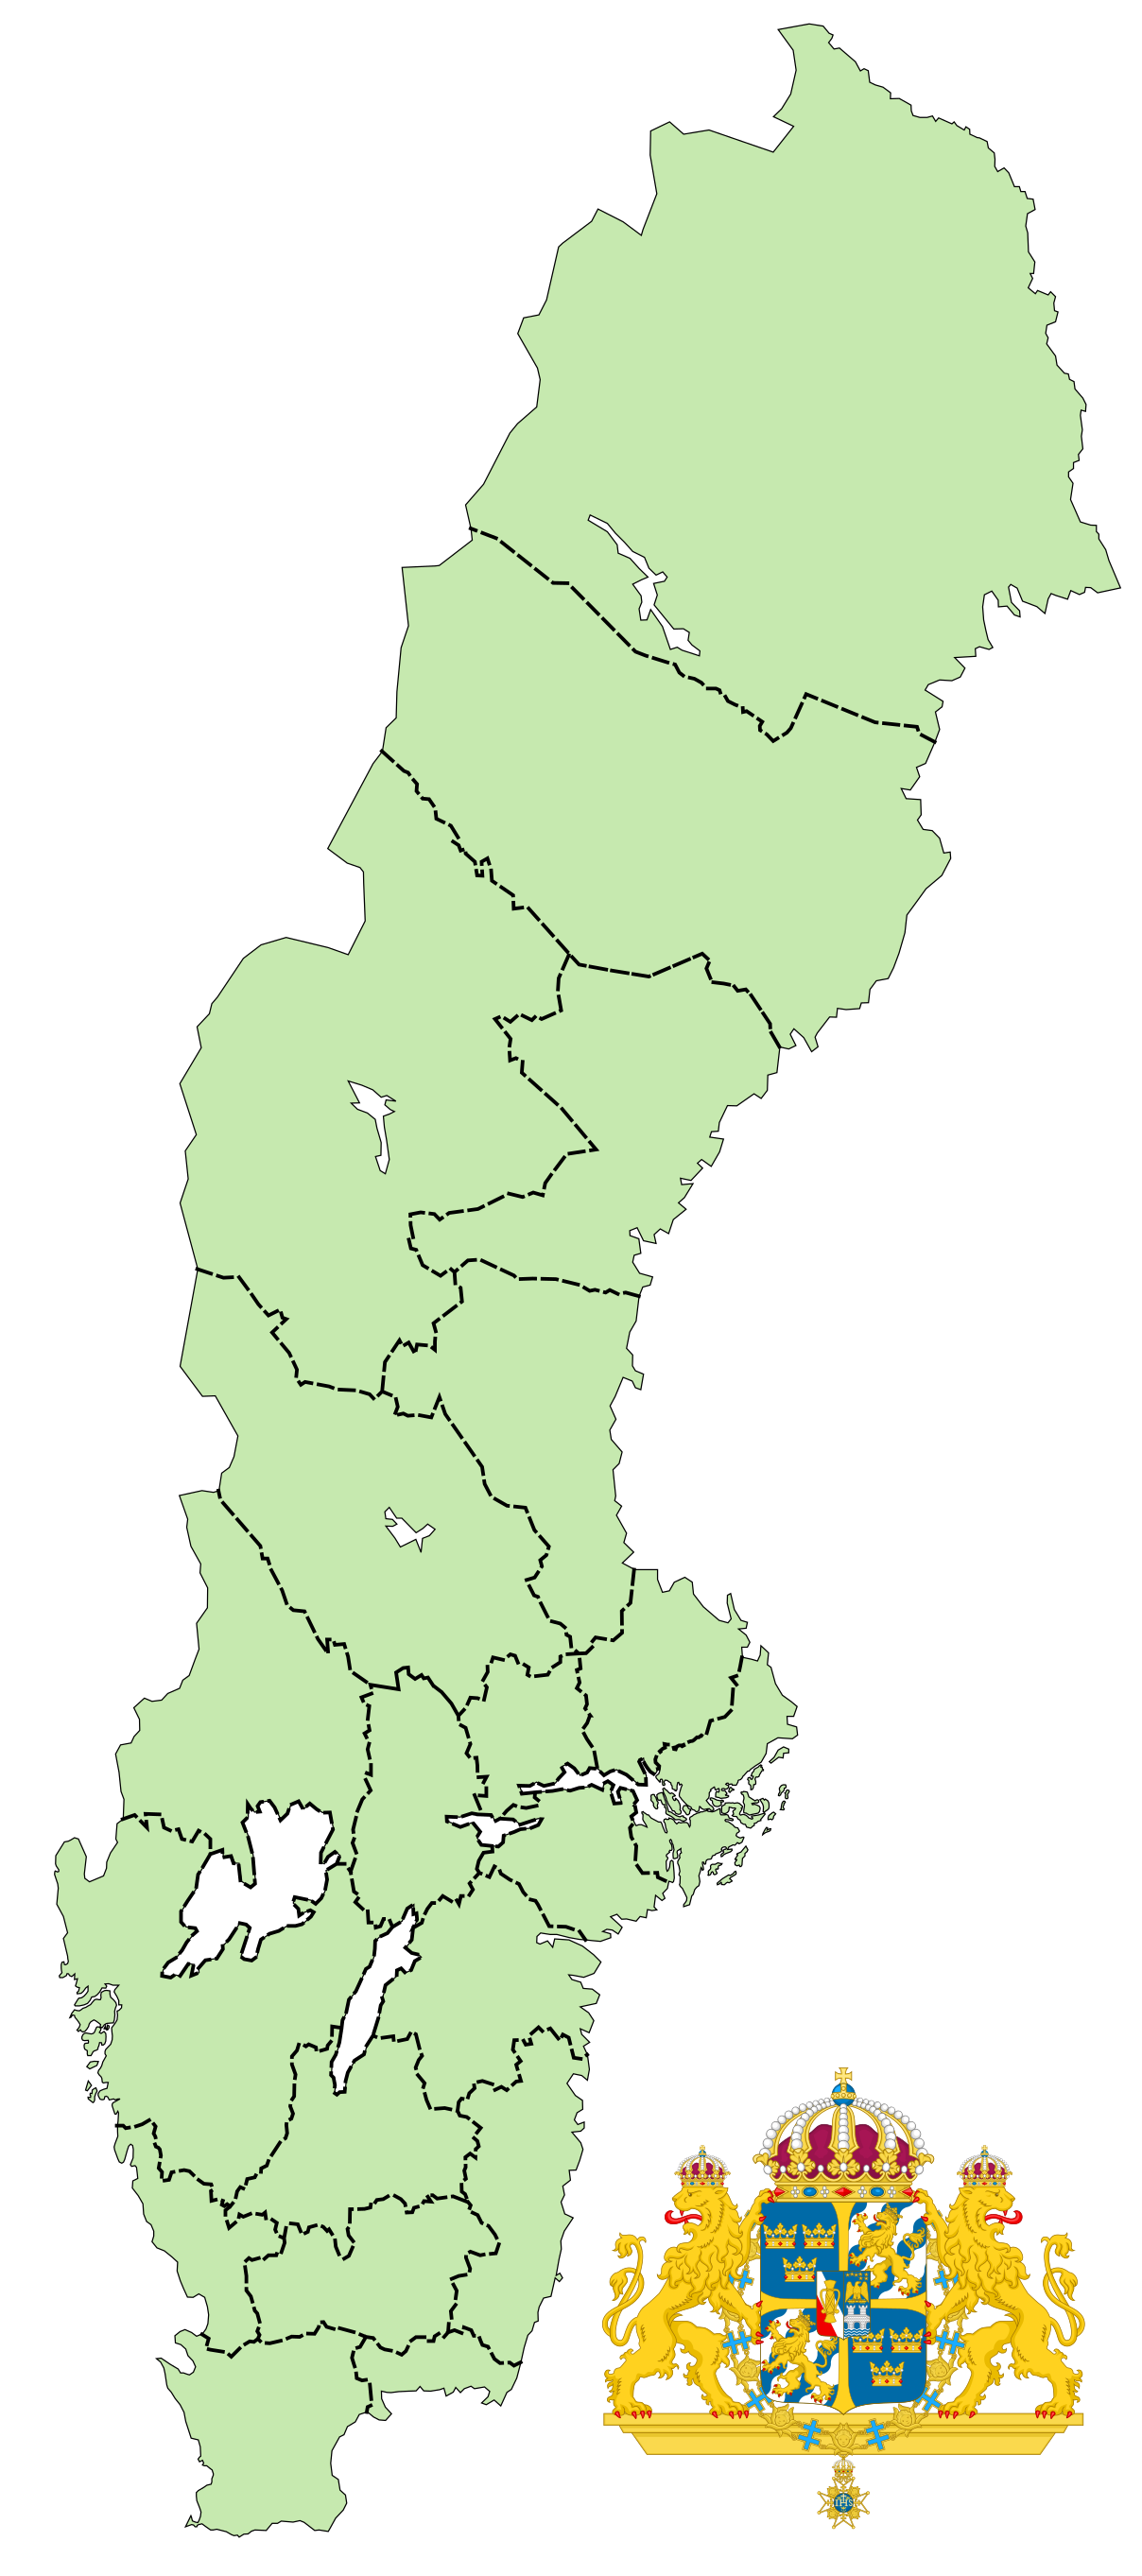
\includegraphics[height=15cm]{LanSverige.png}
\end{center}
\begin{enumerate}[label=\alph*.]
 \item Draw its \textit{dual graph}, which has one vertex for each region, and an edge whenever two regions share a 1d border (not just touch at a point).
%  \item How many domino tilings are there of this dual graph?
\end{enumerate}
 \end{problem}



\begin{problem}
    Examples coming from 3d geometry.
    \begin{enumerate}[label=\alph*.]
         \item Consider the hexagon graph and its dual 
          \begin{center}
    \begin{tikzpicture}
        % Draw the same grid rotated by 120 and 240 degrees around (0,0)
        \foreach \angle in {0,120,240} {
            \begin{scope}[rotate around={\angle:(0,0)}]
                % Draw a 3x3 square grid with 3pt circles at each grid point
                \foreach \x in {0,1,2} {
                    \foreach \y in {0,1,2} {
                        \draw[fill=black] (0.866*\x,{\y - 0.5*\x}) circle (2pt);
                    }
                }
                % Optionally, draw the grid lines
                \foreach \x in {0,1,2} {
                    \draw (0.866*\x,{0- 0.5*\x}) -- (0.866*\x,{2- 0.5*\x});
                }
                \foreach \y in {0,1,2} {
                    \draw (0,\y) -- (0.866*2,{\y- 0.5*2});
                }
                % Draw diagonal edges
                \draw (0,0) -- (0.866*2,2-0.5*2); % (0,0) to (2,2)
                \draw (0.866*1,-0.5) -- (0.866*2,1-0.5*2); % (1,0) to (2,1)
                \draw (0,1) -- (0.866*1,2-0.5*1); % (0,1) to (1,2) \end{scope}
            \end{scope}
        }

        \begin{scope} 
         [xshift = 6cm ]
          \foreach \angle in {0,120,240} {
                \begin{scope}[rotate around={\angle:(0,0)}]
                % Draw a 3x3 square grid with 3pt circles at each grid point
                \foreach \x in {0,1,2} {
                    \foreach \y in {0,1,2} {
                    \draw[fill=black!30, draw=black!30] (0.866*\x,{\y - 0.5*\x}) circle (2pt);
                    }
                }
                % Optionally, draw the grid lines
                \foreach \x in {0,1,2} {
                    \draw[draw=black!30] (0.866*\x,{0- 0.5*\x}) -- (0.866*\x,{2- 0.5*\x});
                }
                \foreach \y in {0,1,2} {
                    \draw[draw=black!30] (0,\y) -- (0.866*2,{\y- 0.5*2});
                }
                % Draw diagonal edges
                \draw[draw=black!30] (0,0) -- (0.866*2,2-0.5*2); % (0,0) to (2,2)
                \draw[draw=black!30] (0.866*1,-0.5) -- (0.866*2,1-0.5*2); % (1,0) to (2,1)
                \draw[draw=black!30] (0,1) -- (0.866*1,2-0.5*1); % (0,1) to (1,2)
                \end{scope}
            }

            \foreach \angle in {0,120,240} {
                \begin{scope}[rotate around={\angle:(0,0)}]
             \foreach \x in {0,1} {
                    \foreach \y in {0.5,1.5} {
                    \fill (0.288+0.866*\x,{\y - 0.5*\x}) circle (2pt);
                    \draw (-0.288+0.866*\x,{\y - 0.5*\x}) -- (0.288+0.866*\x,{\y - 0.5*\x});
                    }
                }
                
             \foreach \x in {0,1} {
                    \foreach \y in {0,1} {
                    \fill (0.866-0.288+0.866*\x,{\y - 0.5*\x}) circle (2pt);
                    \draw (0.866-0.288+0.866*\x,{\y - 0.5*\x}) -- (0.288+0.866*\x,{\y + 0.5 - 0.5*\x});
                    \draw (0.866-0.288+0.866*\x,{\y - 0.5*\x}) -- (0.288+0.866*\x,{\y - 0.5 - 0.5*\x});
                    }
                }
            
            \end{scope}
            } 
         \end{scope}
    \end{tikzpicture}
    \end{center}
       Draw three possible domino tilings of the dual graph, and show that they correspond to colouring in the regions of the hexagonal graph in by \textit{lozenges}
        \begin{center}
        \begin{tikzpicture}
        % Draw a single lozenge (rhombus) with 60 and 120 degree angles
        \draw[thick, fill=orange!30] (0,0) -- (1,0.577) -- (2,0) -- (1,-0.577) -- cycle;
        \node at (4,0) {\textit{lozenge}};
         \end{tikzpicture}
         \end{center}

        \item How many domino tilings are there of the duals to the $2\times2\times2$ and $3\times3\times3$ hexagonal graphs?
        \item Give a 3D geometric description of such a tiling.
        \item If we remove the following region, how many domino tilings are there of the dual graph?
          \begin{center}
    \begin{tikzpicture}
        % Draw the same grid rotated by 120 and 240 degrees around (0,0)
            \foreach \angle in {0,120,240} {
                \begin{scope}[rotate around={\angle:(0,0)}]
                % Draw a 3x3 square grid with 3pt circles at each grid point
                \foreach \x in {0,1,2,3} {
                    \foreach \y in {0,1,2,3} {
                    \draw[fill=black] (0.866*\x,{\y - 0.5*\x}) circle (2pt);
                    }
                }
                % Optionally, draw the grid lines
                \foreach \x in {0,1,2,3} {
                    \draw (0.866*\x,{0- 0.5*\x}) -- (0.866*\x,{3- 0.5*\x});
                }
                \foreach \y in {0,1,2,3} {
                    \draw (0,\y) -- (0.866*3,{\y- 0.5*3});
                }
                % Draw diagonal edges
                \draw (0,0) -- (0.866*3,3-0.5*3); % (0,0) to (3,3)
                \draw (0.866*1,-0.5) -- (0.866*3,2-0.5*3); % (1,0) to (3,2)
                \draw (0,1) -- (0.866*2,3-0.5*2); % (0,1) to (2,3)
                % Add edges from (0,2) to (1,3) and from (2,0) to (3,1)
                \draw (0.866*0,2-0.5*0) -- (0.866*1,3-0.5*1);
                \draw (0.866*2,0-0.5*2) -- (0.866*3,1-0.5*3);
                \end{scope}
            }

            \fill[pattern=north east lines] 
                (0.866*1,1-0.5*1) -- 
                (0.866*3,1-0.5*3) -- 
                (0.866*3,3-0.5*3) -- 
                (0.866*1,3-0.5*1) -- 
                cycle;

            \fill[pattern=north west lines] 
                (0.866*0, -3-0.5*0) -- 
                (0.866*1, -2-0.5*1) -- 
                (0.866*-2, -2-0.5*-2) -- 
                (0.866*-2, 1-0.5*-2) -- 
                (0.866*-3, 0-0.5*-3) -- 
                (0.866*-3, -3-0.5*-3) -- 
                cycle;
    \end{tikzpicture}
    \end{center}
    \end{enumerate}
\end{problem}










    % \begin{center}
    % \begin{tikzpicture}
    %     % Draw the same grid rotated by 120 and 240 degrees around (0,0)
    %     \foreach \angle in {0,120,240} {
    %         \begin{scope}[rotate around={\angle:(0,0)}]
    %             % Draw a 3x3 square grid with 3pt circles at each grid point
    %             \foreach \x in {0,1,2} {
    %                 \foreach \y in {0,1,2} {
    %                     \draw[fill=black] (0.866*\x,{\y - 0.5*\x}) circle (2pt);
    %                 }
    %             }
    %             % Optionally, draw the grid lines
    %             \foreach \x in {0,1,2} {
    %                 \draw (0.866*\x,{0- 0.5*\x}) -- (0.866*\x,{2- 0.5*\x});
    %             }
    %             \foreach \y in {0,1,2} {
    %                 \draw (0,\y) -- (0.866*2,{\y- 0.5*2});
    %             }
    %         \end{scope}

    %         % y (0,1)   x (0.5,0.866)
    %     }

    % \end{tikzpicture}
    % \end{center}










    

\newpage
    \chapter{Random domino tilings}
\kapiteldatum{2 July}


\setcounter{problem}{0}


\begin{definition}
    A \emph{random domino tiling} of a finite region is a probability distribution (on the set of all tilings) where each domino tiling $T$ is equally likely
    $$\mathbf{P}(\textup{tiling }T) \ = \ \frac{1}{\#\{\textup{all tilings }T'\}}.$$
\end{definition}



\begin{problem}
    Random domino tilings of  $2\times n$ rectangle.
        \begin{center}
        \begin{tikzpicture}
        % Draw grid
        \foreach \x in {1,...,12} {
            \draw[dashed, opacity=0.3] (\x,0) -- (\x,4);
        }
        \foreach \y in {1,...,3} {
            \draw[dashed, opacity=0.3] (0,\y) -- (13,\y);
        }
        % Draw blue region: 2x6 rectangle from (1,1) to (7,3)
        \filldraw[fill=blue, opacity=0.1, ultra thick] (1,1) -- (12,1) -- (12,3) -- (1,3) -- cycle;
        \end{tikzpicture}
        \end{center}
   \begin{enumerate}[label=\alph*.]
    \item Draw all domino tilings of the $2\times 5$ rectangle. Compute the probability that the leftmost domino is vertical.
    \item What is the answer for the $2\times n$ rectangles?
    \item If the leftmost domino of an $2\times n$ rectangle is vertical, what is the probability that the rightmost domino is vertical? 
    \item What is the limit of b. and c. as $n\to\infty$?
   \end{enumerate}
\end{problem}

\begin{problem}
   Take a domino tiling, and consider the sequence of boxes, labelled by $k=1,\ldots ,n-1$.
   
        \begin{center}
        \begin{tikzpicture}
            % Draw grid
            \foreach \x in {1,...,12} {
                \draw[dashed, opacity=0.3] (\x,0) -- (\x,4);
            }
            \foreach \y in {1,...,3} {
                \draw[dashed, opacity=0.3] (0,\y) -- (13,\y);
            }
            % Draw green dominos (vertical and horizontal tiling by hand)
            % First row: vertical, horizontal
            \filldraw[fill=green, fill opacity=0.3] (1,1) rectangle (2,3); % vertical at (1,1)-(2,3)
            \filldraw[fill=green, fill opacity=0.3] (2,1) rectangle (4,2); % horizontal at (2,1)-(4,2)
            % Second row: vertical, vertical, vertical
            \filldraw[fill=green, fill opacity=0.3] (2,2) rectangle (4,3); % vertical at (2,2)-(3,4)
            \filldraw[fill=green, fill opacity=0.3] (4,1) rectangle (5,3); % vertical at (4,1)-(5,3)
            % Third row: horizontal, horizontal, vertical
            \filldraw[fill=green, fill opacity=0.3] (5,1) rectangle (6,3); % horizontal at (5,1)-(7,2)
            \filldraw[fill=green, fill opacity=0.3] (6,1) rectangle (7,3); % vertical at (6,1)-(7,3)
            \filldraw[fill=green, fill opacity=0.3] (7,2) rectangle (9,3); % horizontal at (7,2)-(9,3)
            \filldraw[fill=green, fill opacity=0.3] (7,1) rectangle (9,2); % horizontal at (7,1)-(9,2)
            \filldraw[fill=green, fill opacity=0.3] (9,1) rectangle (10,3); % vertical at (9,1)-(10,3)
            \filldraw[fill=green, fill opacity=0.3] (10,1) rectangle (11,3); % vertical at (10,1)-(11,3)
            \filldraw[fill=green, fill opacity=0.3] (11,1) rectangle (12,3); % vertical at (11,1)-(12,3)

            \draw[ultra thick, red] (3,1) rectangle (5,3); % vertical line at x=3
            \draw[line width = 3pt, red] (3,0.75) rectangle (3,3.25); % vertical line at x=3
            \node at (3.5,3.5) {$k$}; % Label for k
            \node at (1.5,3.5) {$1$}; % Label for k
            \node at (11.5,3.5) {$n$}; % Label for k
        \end{tikzpicture}
        \end{center}
\begin{enumerate}[label=\alph*.]
    \item Let $f:\{0,1, \ldots ,n\}\to \{0,2\}$ be the function counting the number of horizontal dominoes completely contained in the $k$th box. Show that $f$ uniquely determines the domino tiling.
    \item Give a bijection between domino tilings of the $2\times n$ rectangle and maximal paths on the following graph:
        \begin{center}
        \begin{tikzpicture}
            % Draw grid
            \foreach \x in {0,...,13} {
                \draw[dashed, opacity=0.3] (\x,0) -- (\x,4);
            }
            \node at (3.5,3.5) {$k$}; % Label for k
            \node at (1.5,3.5) {$1$}; % Label for k
            \node at (10.5,3.5) {$n-1$}; % Label for k

            % For each column, draw two dots (no labels)
            \foreach \k in {1,...,10} {
                % Draw dots at (k+0.5,2) and (k+0.5,1)
                \fill (\k+0.5,2) circle (2pt);
                \fill (\k+0.5,1) circle (2pt);
                % Node above top dot
                \node[above] at (\k+0.5,2) {0};
                % Node below bottom dot
                \node[below] at (\k+0.5,1) {2};
                % Draw edges if not the last column
                \ifnum\k<10
                        % Edge from (k+0.5,2) to (k+1.5,2)
                        \draw[->, shorten >=4pt, shorten <=4pt]  (\k+0.5,2) -- (\k+1.5,2);
                        % Edge from (k+0.5,2) to (k+1.5,1)
                        \draw[->, shorten >=4pt, shorten <=4pt]  (\k+0.5,2) -- (\k+1.5,1);
                        % Edge from (k+0.5,1) to (k+1.5,2)
                        \draw[->, shorten >=4pt, shorten <=4pt]  (\k+0.5,1) -- (\k+1.5,2);
                \fi
            }
        \end{tikzpicture}
        \end{center}
     \item Give another proof that this is the $n$th Fibonacci number.
    \item \textit{Attempt if you know matrices.} Define the matrix 
    $$M \ = \ \begin{pmatrix} 
     1 &1 \\ 
     1 &0 
     \end{pmatrix}.$$
     Show that the number of domino tilings of the $2\times n$ rectangle is equal to the top left entry $a_n$ of $M^n=M\times \cdots\times M$. 
     \item \textit{Attempt if you know matrices.} Show that 
     $$M^2 \ = \ M + 1$$
     hence show that $a_{n+2} = a_{n+1} + a_n$.
     \item \textit{Attempt if you know matrices.} Consider the top-left entry $b_n\in \mathbf{Z}[x,y]$ of $N^n$, for the matrix
     $$N \ = \ \begin{pmatrix} 
     x &y \\ 
     y &0 
     \end{pmatrix}.$$
     Compute $b_1,b_2,b_3,b_4$. What is the interpretation of the $x^iy^j$-coefficient of $b_n$? Show that $b_{n+2} = x b_{n+1} + y^2 b_n$. Find a formula for $b_n$ of the form 
     $$b_n \ = \ c_1 \cdot \varphi_1^n + c_2 \cdot \varphi_2^n.$$
     \textit{Hint: find two solutions of the form $\varphi_i^n$, to the equation, then use $b_1,b_2$ to find $c_1,c_2$. }
\end{enumerate}
\end{problem}


\begin{definition}
    A \emph{walk} on a graph $G$ is a sequence of vertices $v_0,v_1, \ldots ,v_t$, where each vertex is adjacent to the next. A \emph{random walk} is a probability distribution on the set of all walks, where each walk is equally likely, 
    $$\mathbf{P}(\textup{walk }v_0, \ldots ,v_t) \ = \ \frac{1}{\#\{\textup{all walks }\}}.$$
\end{definition}

One can similarly define a \textit{random walk starting at a fixed vertex $v$}, or a random walk with some other set of properties.


\begin{problem}
  Random walks. Consider a random walk on $\mathbf{Z}$ of length $t$, which we draw as a path in $\mathbf{Z}\times \{0,1, \ldots ,t\}$.
  \begin{center}
    \begin{tikzpicture}
% Draw a 10x6 grid with dots at half-integer spacing
\foreach \x in {0,...,20} {
    \foreach \y in {0,...,10} {
    % Colour: middle rows (y=1..9) black!40, outer rows (y=0,10) black!20
        \ifnum\y=0
            \fill[fill=black!15] (0.3*\x,0.3*\y+0.3) circle (2pt);
        \else\ifnum\y=10
            \fill[fill=black!15] (0.3*\x,0.3*\y+0.3) circle (2pt);
        \else
            \fill[fill=black!40] (0.3*\x,0.3*\y+0.3) circle (2pt);
        \fi\fi
    }
} 

% Draw a red path starting at (0,0), mapped to (0,6)
% Generate a random walk: start at y=6, each step increases or decreases by 1 randomly
\draw[very thick, red]
    (0*0.3, 6*0.3)
    \foreach \x/\y in {1/7, 2/6, 3/7, 4/8, 5/7, 6/6, 7/5, 8/6, 9/7, 10/6, 11/7, 12/8, 13/7, 14/8, 15/7, 16/6, 17/7, 18/6, 19/5, 20/4} {
        -- (\x*0.3, \y*0.3)
    };

    \node at (21*0.3,6*0.3) {\textcolor{red}{$\gamma$}};
        \end{tikzpicture}
   \end{center}
\begin{enumerate}[label=\alph*.]
 \item How many walks of length $t$ are there? 
 \item What is the probability that a random walk $\gamma$ has $\gamma(t) \ge 0$?
 \item What is $\mathbf{E}(\gamma(t))$?
 \item What is $\mathbf{E}(\gamma(t)^2)$? In plain English, approximately how far away from the origin should we expect $\gamma$ to be after $t$ steps?
\end{enumerate}
\end{problem}


\begin{problem}
  Show that the set of tilings of the $1\times B\times C$ hexagon by lozenges
\begin{center}
\begin{tikzpicture}

        % Draw orange lozenges at specified positions
        \foreach \x/\y in {-2/-2, -1/-2, 0/-1, -1/0} {
            \pgfmathsetmacro{\cx}{0.866*\x}
            \pgfmathsetmacro{\cy}{\y - 0.5*\x}
            \begin{scope}[shift={(\cx,\cy)}]
            \draw[thick, fill=orange!30] (0,0) -- (0.866,0.5) -- (1.732,0) -- (0.866,-0.5) -- cycle;
            \end{scope}
        }
     \foreach \x/\y in { -2/-2, 0/-1} {
            \pgfmathsetmacro{\cx}{0.866*\x}
            \pgfmathsetmacro{\cy}{\y - 0.5*\x}
            \begin{scope}[shift={(\cx,\cy)}]
                \begin{scope}[rotate around={60:(0,0)}]
            \draw[thick, fill=blue!30] (0,0) -- (0.866,0.5) -- (1.732,0) -- (0.866,-0.5) -- cycle;
                \end{scope}
            \end{scope}
        }
     \foreach \x/\y in {0/-1, 2/0} {
            \pgfmathsetmacro{\cx}{0.866*\x}
            \pgfmathsetmacro{\cy}{\y - 0.5*\x}
            \begin{scope}[shift={(\cx,\cy)}]
                \begin{scope}[rotate around={120:(0,0)}]
            \draw[thick, fill=green!30] (0,0) -- (0.866,0.5) -- (1.732,0) -- (0.866,-0.5) -- cycle;
                \end{scope}
            \end{scope}
        }


    \node[left] at ({0.866*(-2)},{-1.5 - 0.5*(-2)}) {$1$};
    \node[above] at ({0.866*(-1)},{0 - 0.5*(-1)}) {$B$};
    \node[above] at ({0.866*1},{1 - 0.5*1}) {$C$};


\end{tikzpicture}
 \end{center} 
 is equivalent to a certain set of walks in $\mathbf{Z}$ (which you should define precisely).

 \begin{enumerate}[label =\alph*.]
  \item Picking a random tiling (or equivalently, a random walk), what is the expected number of 3d cubes in a random $1\times B\times C$ lozenge tiling?
  \item Given a tiling $T$ on the hexagonal graph $G$, we define the \textit{height function} 
  $$h_T \ : \ V(G) \ \to \ \mathbf{N}$$
  whose value is the number of 3d boxes under ($\downarrow$) that vertex. Describe the walk attached to $T$ in terms of $h_T$.
  \item \textit{If you're interested in continuing, try the lattice paths long problem.}
 \end{enumerate}
\end{problem}


% \begin{problem}
%   Dominoes and paths.  
%           \begin{center}
%         \begin{tikzpicture}
%             % Draw grid for 3x12 rectangle
%             \foreach \x in {1,...,11} {
%                 \draw[dashed, opacity=0.3] (\x,0) -- (\x,5);
%             }
%             \foreach \y in {1,...,4} {
%                 \draw[dashed, opacity=0.3] (0,\y) -- (12,\y);
%             }
%             % Example domino tiling for 3x12 rectangle
%             % First column: vertical domino
%             \filldraw[fill=green, fill opacity=0.3] (1,1) rectangle (2,3);
%             \filldraw[fill=green, fill opacity=0.3] (1,3) rectangle (3,4);
%             % Next two columns: three horizontal dominoes (should be 2x1)
%             \filldraw[fill=green, fill opacity=0.3] (2,1) rectangle (4,2);
%             \filldraw[fill=green, fill opacity=0.3] (2,2) rectangle (4,3);
%             \filldraw[fill=green, fill opacity=0.3] (3,3) rectangle (5,4);

%             % Draw horizontal dominoes with bottom left at (4,1), (4,2), (5,3)
%             \filldraw[fill=green, fill opacity=0.3] (4,1) rectangle (6,2);
%             \filldraw[fill=green, fill opacity=0.3] (4,2) rectangle (6,3);
%             \filldraw[fill=green, fill opacity=0.3] (5,3) rectangle (7,4);

%             % Draw vertical domino with bottom left at (6,1)
%             \filldraw[fill=green, fill opacity=0.3] (6,1) rectangle (7,3);

%             % Draw three horizontal dominoes with bottom left at (7,1), (7,2), (7,3)
%             \filldraw[fill=green, fill opacity=0.3] (7,1) rectangle (9,2);
%             \filldraw[fill=green, fill opacity=0.3] (7,2) rectangle (9,3);
%             \filldraw[fill=green, fill opacity=0.3] (7,3) rectangle (9,4);

%             % Draw one horizontal domino at the bottom with x=9 (from (9,1) to (11,2))
%             \filldraw[fill=green, fill opacity=0.3] (9,1) rectangle (11,2);

%             % Draw two vertical dominoes over it at (9,2)-(10,4) and (10,2)-(11,4)
%             \filldraw[fill=green, fill opacity=0.3] (9,2) rectangle (10,4);
%             \filldraw[fill=green, fill opacity=0.3] (10,2) rectangle (11,4);

%             % Mark some vertical line at x=3 for k
%             \draw[ultra thick, red] (3.5,0.75) -- (3.5,4.25);
%             \node at (3.5,4.5) {$k$};
%             \node at (1.5,4.5) {$1$};
%             \node at (10.5,4.5) {$n$};
%         \end{tikzpicture}
%         \end{center}
%     A \textit{state} at a vertical slice is the set of all dominoes touching the slice. 
% \begin{enumerate}[label = \alph*.]
%  \item Show that there are $12$ possible states, thus show that the map $f:\{1,2, \ldots ,n\} \to \{S_1, S_2, \ldots , S_{12}\}$ uniquely determines the domino tiling. Can you come up with a smaller set that also uniquely determines the domino tiling?
% \end{enumerate}
% \end{problem}





















\newpage 
 \chapter{Random dominoes 3}
\kapiteldatum{3 July}




\setcounter{problem}{0}

\textbf{Probability.}

\begin{definition}
  A \textit{probability space} is a countable (i.e. finite or has as many elements as $\textbf{N}$) set $\Omega$ together with a function 
  $$\mathbf{P}\ : \ \{\textup{subsets of }\Omega\} \ \to \ [0,1]$$
  such that 
  \begin{enumerate}
   \item $\mathbf{P}(\Omega)=1$, 
   \item if $A_1, A_2 \ldots$ are disjoint subsets of $\Omega$, then $\mathbf{P}(A_1 \cup A_2 \cup \cdots \ ) = \mathbf{P}(A_1)+\mathbf{P}(A_2)+\cdots$ .
  \end{enumerate}
If $X:\Omega \to \mathbf{R}$ is a function, its \textit{expectation} is defined to be 
$$\mathbf{E}(X) \ = \ \sum_{a\in \Omega} \mathbf{P}(\{a\})\cdot X(a).$$
A function $X$ is called a \textit{random variable}, or a \textit{random real number}.
\end{definition}


\begin{problem}
Consider one white and one black 6-sided dice, both with faces numbered $1,2,3,4,5,6$. 
\begin{center}
\begin{tikzpicture}
% Draw a small square for the die
\draw[thick, fill=white] (0,0) rectangle (0.5,0.5);
% Draw five small dots: four in the corners, one in the center
\foreach \x/\y in {0.1/0.1, 0.4/0.1, 0.1/0.4, 0.4/0.4} {
    \fill ( \x, \y ) circle (0.05cm);
}
\fill (0.25,0.25) circle (0.05cm);

% Draw a small square for the black die, shifted to the right
\begin{scope}[xshift=1.2cm]
\draw[thick, fill=black] (0,0) rectangle (0.5,0.5);
% Draw four white dots in the corners
\foreach \x/\y in {0.1/0.1, 0.4/0.1, 0.1/0.4, 0.4/0.4} {
    \fill[white] ( \x, \y ) circle (0.05cm);
}
\end{scope}
 \end{tikzpicture}
 \end{center} 
\begin{enumerate}[label =\alph*.]
 \item Draw the set $\Omega$ of possible outcomes of rolling the two dice (in a $6 \times 6$ table).
 \item Let $W,B:\Omega \to \mathbf{R}$ denote the values of the white and black dice, respectively. What are the expectations
 $$\mathbf{E}(W), \ \mathbf{E}(B), \ \mathbf{E}(10 W + 2B)?$$
 What are \textit{variances} 
 $$\mathbf{E}((W-\mathbf{E}(W))^2), \ \mathbf{E}((B-\mathbf{E}(B))^2), \ \mathbf{E}((10 W + 2B - \mathbf{E}(10 W + 2B))^2)?$$
 Write down on paper a plain English/Swedish description of what this means.
 \item The \textit{correlator}
 $$\mathbf{E}\left( (W - \mathbf{E}(W))(B-\mathbf{E}(B))\right)$$
 measures how much information you get about the value $W(a)$ if you know the value $B(a)$, and vice versa. Draw the values of the function 
 $$(W - \mathbf{E}(W))(B-\mathbf{E}(B)) \ : \ \Omega \ \to \ \mathbf{R}$$
 on the $6\times 6$ table. What is the value of this correlator?
 \item The dice are now enchanted, so that the rolls are never more than $4$ apart. Other than that all pairs of rolls are equally likely. What is the new answer to a., b. and c.?
\end{enumerate}


 
\end{problem}





\textbf{Back to random domino tilings.}

\begin{problem}
  Correlators. In the following $\Omega$ will be the set of all lozenge tilings of a certain region, and the value of $\mathbf{P}$ is the same for each tiling.

\begin{center}
\begin{tikzpicture}
        % Draw orange lozenges at specified positions
        \foreach \x/\y in {-2/-2, -1/-2, 0/-1, -1/0} {
            \pgfmathsetmacro{\cx}{0.866*\x}
            \pgfmathsetmacro{\cy}{\y - 0.5*\x}
            \begin{scope}[shift={(\cx,\cy)}]
            \draw[thick, fill=orange!30] (0,0) -- (0.866,0.5) -- (1.732,0) -- (0.866,-0.5) -- cycle;
            \end{scope}
        }
     \foreach \x/\y in {-1/0, -2/-1, -2/-2, 0/-1} {
            \pgfmathsetmacro{\cx}{0.866*\x}
            \pgfmathsetmacro{\cy}{\y - 0.5*\x}
            \begin{scope}[shift={(\cx,\cy)}]
                \begin{scope}[rotate around={60:(0,0)}]
            \draw[thick, fill=blue!30] (0,0) -- (0.866,0.5) -- (1.732,0) -- (0.866,-0.5) -- cycle;
                \end{scope}
            \end{scope}
        }
     \foreach \x/\y in {0/-1, 2/0, 2/1, 1/1} {
            \pgfmathsetmacro{\cx}{0.866*\x}
            \pgfmathsetmacro{\cy}{\y - 0.5*\x}
            \begin{scope}[shift={(\cx,\cy)}]
                \begin{scope}[rotate around={120:(0,0)}]
            \draw[thick, fill=green!30] (0,0) -- (0.866,0.5) -- (1.732,0) -- (0.866,-0.5) -- cycle;
                \end{scope}
            \end{scope}
        }

    % Mark points (2,1) and (2,2) in hexagonal coordinates as red filled circles
    \foreach \x/\y in {1/1, 0/1} {
        \pgfmathsetmacro{\cx}{0.866*\x}
        \pgfmathsetmacro{\cy}{\y - 0.5*\x}
        \fill[red] (\cx,\cy) circle (3pt);
    }
    \node[right, red] at ({0.866*1},{1 - 0.5*1 + 0.3}) {$y$};
    \node[right, red] at ({0.866*0},{0 + 0.5*1 + 0.3}) {$x$};

    \begin{scope} 
     [xshift=-0.2cm] 
    \node at ({0},{2}) {$2$};
    \node at ({0},{1}) {$1$};
    \node at ({0},{0}) {$1$};
    \node at ({0},{-1}) {$0$};
    \node at ({0},{-2}) {$0$};

    \node at ({0.866*-2},{2-1}) {$2$};
    \node at ({0.866*-2},{1-1}) {$1$};
    \node at ({0.866*-2},{0-1}) {$0$};
     \end{scope}

 \end{tikzpicture}
 \end{center} 
 \begin{enumerate}[label =\alph*.]
  \item Show that there are 20 lozenge tilings of the $2\times 2 \times 2$ hexagon. 
  \item Write down the \textit{height function} $h_T:V(G)\to \mathbf{N}$ of two tilings $T$. Here $V(G)$ is the vertex set of  the hexagonal graph, some heights are given above for the above tiling.
  \item What are the expected values $\textbf{E}(h_T(x))$ and $\textbf{E}(h_T(y))$ for a random tiling $T$?
  \item What is the value of the \textit{correlator} 
   $$C(x,y) \ = \ \textbf{E}(h_T(x)h_T(y)) - \textbf{E}(h_T(x))\textbf{E}(h_T(y))$$
   for the two points $x,y$?
 \end{enumerate}
\end{problem}














\newpage 
 \chapter{Random dominoes 4}
\kapiteldatum{4 July 2025}


\setcounter{problem}{0}

\textit{We'll begin with a proof that lozenge tilings of the $A\times B \times C$ hexagonal graph biject with 3d cube stackings of the $A\times B\times C$ 3d box. Be careful - it's not true if for certain subgraphs of the hexagonal graph!}

\begin{center}
\begin{tikzpicture}
 
        % Draw the same grid rotated by 120 and 240 degrees around (0,0)
        \foreach \angle/\ca/\cb/\cc in {0/blue!30/green!30/orange!30,240/green!30/orange!30/blue!30,120/orange!30/blue!30/green!30} {
            \begin{scope}[rotate around={\angle:(0,0)}]

            % Draw blue rhombi at (1,0), (1,-1), (1,-2) in hexagon coordinates
            \foreach \x/\y in {1/1, 1/0, 1/-1, 1/-2} {
                \pgfmathsetmacro{\cx}{0.866*\x}
                \pgfmathsetmacro{\cy}{\y - 0.5*\x}
                \begin{scope}[shift={(\cx,\cy)}]
                    \begin{scope}[rotate around={60:(0,0)}]
                        \draw[thick, fill=\ca] (0,0) -- (0.866,0.5) -- (1.732,0) -- (0.866,-0.5) -- cycle;
                    \end{scope}
                \end{scope}
            }

            % Draw green rhombi at (2,1), (2,0), (2,-1), (2,-2) in hexagon coordinates
            \foreach \x/\y in {3/2,3/1, 3/0, 3/-1} {
                \pgfmathsetmacro{\cx}{0.866*\x}
                \pgfmathsetmacro{\cy}{\y - 0.5*\x}
                \begin{scope}[shift={(\cx,\cy)}]
                    \begin{scope}[rotate around={120:(0,0)}]
                        \draw[thick, fill=\cb] (0,0) -- (0.866,0.5) -- (1.732,0) -- (0.866,-0.5) -- cycle;
                    \end{scope}
                \end{scope}
            }

                % Draw orange rhombi at (1,-2) and (-1,-2) in hexagon coordinates
                \foreach \x/\y in {1/-2, 0/-3} {
                    \pgfmathsetmacro{\cx}{0.866*\x}
                    \pgfmathsetmacro{\cy}{\y - 0.5*\x}
                    \begin{scope}[shift={(\cx,\cy)}]
                        \draw[thick, fill=\cc] (0,0) -- (0.866,0.5) -- (1.732,0) -- (0.866,-0.5) -- cycle;
                    \end{scope}
                }


            \end{scope}
        }
    %     % Draw orange lozenges at specified positions
    %     \foreach \x/\y in {-2/-2, -1/-2, 0/-1, -1/0} {
    %         \pgfmathsetmacro{\cx}{0.866*\x}
    %         \pgfmathsetmacro{\cy}{\y - 0.5*\x}
    %         \begin{scope}[shift={(\cx,\cy)}]
    %         \draw[thick, fill=orange!30] (0,0) -- (0.866,0.5) -- (1.732,0) -- (0.866,-0.5) -- cycle;
    %         \end{scope}
    %     }
    %  \foreach \x/\y in {-1/0, -2/-1, -2/-2, 0/-1} {
    %         \pgfmathsetmacro{\cx}{0.866*\x}
    %         \pgfmathsetmacro{\cy}{\y - 0.5*\x}
    %         \begin{scope}[shift={(\cx,\cy)}]
    %             \begin{scope}[rotate around={60:(0,0)}]
    %         \draw[thick, fill=blue!30] (0,0) -- (0.866,0.5) -- (1.732,0) -- (0.866,-0.5) -- cycle;
    %             \end{scope}
    %         \end{scope}
    %     }
    %  \foreach \x/\y in {0/-1, 2/0, 2/1, 1/1} {
    %         \pgfmathsetmacro{\cx}{0.866*\x}
    %         \pgfmathsetmacro{\cy}{\y - 0.5*\x}
    %         \begin{scope}[shift={(\cx,\cy)}]
    %             \begin{scope}[rotate around={120:(0,0)}]
    %         \draw[thick, fill=green!30] (0,0) -- (0.866,0.5) -- (1.732,0) -- (0.866,-0.5) -- cycle;
    %             \end{scope}
    %         \end{scope}
    %     }

\end{tikzpicture}
 \end{center}




\begin{problem} Hexagonal paths.
    \begin{enumerate}[label =\alph*.]
     \item Give a bijection between tilings of the $A\times B \times C$ hexagon and certain a certain set of paths in $\mathbf{Z}^2$ (which you should precisely specify).
   
\begin{center}
\begin{tikzpicture}
 
        % Draw the same grid rotated by 120 and 240 degrees around (0,0)
        \foreach \angle in {0,120,240} {
            \begin{scope}[rotate around={\angle:(0,0)}]
                % Draw a 3x3 square grid with 3pt circles at each grid point
                % \foreach \x in {0,1,2} {
                %     \foreach \y in {0,1,2} {
                %         \draw[fill=black] (0.866*\x,{\y - 0.5*\x}) circle (2pt);
                %     }
                % }
                % Optionally, draw the grid lines
                \foreach \x in {0,1,2} {
                    \draw (0.866*\x,{0- 0.5*\x}) -- (0.866*\x,{2- 0.5*\x});
                }
                \foreach \y in {0,1,2} {
                    \draw (0,\y) -- (0.866*2,{\y- 0.5*2});
                }
                % Draw diagonal edges
                \draw (0,0) -- (0.866*2,2-0.5*2); % (0,0) to (2,2)
                \draw (0.866*1,-0.5) -- (0.866*2,1-0.5*2); % (1,0) to (2,1)
                \draw (0,1) -- (0.866*1,2-0.5*1); % (0,1) to (1,2) 
            \end{scope}
        }
        % Draw orange lozenges at specified positions
        \foreach \x/\y in {-2/-2, -1/-2, 0/-1, -1/0} {
            \pgfmathsetmacro{\cx}{0.866*\x}
            \pgfmathsetmacro{\cy}{\y - 0.5*\x}
            \begin{scope}[shift={(\cx,\cy)}]
            \draw[thick, fill=orange!30] (0,0) -- (0.866,0.5) -- (1.732,0) -- (0.866,-0.5) -- cycle;
            \end{scope}
        }
     \foreach \x/\y in {-1/0, -2/-1, -2/-2, 0/-1} {
            \pgfmathsetmacro{\cx}{0.866*\x}
            \pgfmathsetmacro{\cy}{\y - 0.5*\x}
            \begin{scope}[shift={(\cx,\cy)}]
                \begin{scope}[rotate around={60:(0,0)}]
            \draw[thick, fill=blue!30] (0,0) -- (0.866,0.5) -- (1.732,0) -- (0.866,-0.5) -- cycle;
                \end{scope}
            \end{scope}
        }
     \foreach \x/\y in {0/-1, 2/0, 2/1, 1/1} {
            \pgfmathsetmacro{\cx}{0.866*\x}
            \pgfmathsetmacro{\cy}{\y - 0.5*\x}
            \begin{scope}[shift={(\cx,\cy)}]
                \begin{scope}[rotate around={120:(0,0)}]
            \draw[thick, fill=green!30] (0,0) -- (0.866,0.5) -- (1.732,0) -- (0.866,-0.5) -- cycle;
                \end{scope}
            \end{scope}
        }

    % Draw two red paths
    \draw[very thick, red] 
        ({0.866*(-2)},{-0.5 - 0.5*(-2)}) -- ({0.866*0},{1.5 - 0.5*0}) -- ({0.866*2},{1.5 - 0.5*2});

    \draw[very thick, red] 
        ({0.866*(-2)},{-1.5 - 0.5*(-2)}) -- ({0.866*(-1)},{-0.5 - 0.5*(-1)}) -- ({0.866*0},{-0.5 - 0.5*0}) -- ({0.866*1},{0.5 - 0.5*1}) -- ({0.866*2},{0.5 - 0.5*2});

    \node[left] at ({0.866*(-2)},{-1 - 0.5*(-2)}) {$A$};
    \node[above] at ({0.866*(-1)},{1 - 0.5*(-1)}) {$B$};
    \node[above] at ({0.866*1},{2 - 0.5*1}) {$C$};

    \begin{scope} 
     [xshift= 5cm,yshift=-1.5cm,scale=0.7]
        
    % Draw a 5x5 dashed grid
    \foreach \x in {0,...,4} {
        \draw[dashed, opacity=0.3] (\x,0) -- (\x,4);
    }
    \foreach \y in {0,...,4} {
        \draw[dashed, opacity=0.3] (0,\y) -- (4,\y);
    } 
    % Draw two red paths
    \draw[very thick, red] (0,1) -- (1,2) -- (2,3) -- (4,3);
    % Second path: (0,1) -- (4,4)
    \draw[very thick, red] (0,0) -- (1,1) -- (2,1) -- (3,2) -- (4,2);

    % Draw nodes for gamma_1 and gamma_2 to the right of the end of both paths
    \node[right, red] at (4,3) {$\gamma_1$};
    \node[right, red] at (4,2.5) {$\cdots$};
    \node[right, red] at (4,2) {$\gamma_A$};

    \node[below] at (2,0) {$p$};


\end{scope}

\end{tikzpicture}
 \end{center}
 \item  What are the graphs corresponding to the lozenge tilings with the maximum and minimum number of 3d boxes?
 \item  How can you see the number of 3d boxes from the paths?
 \item  What is the expected value of $\gamma_1(p), \ldots, \gamma_A(p)$ for the $2\times 2\times 2$ hexagon?
    \end{enumerate}
In the next problem we will find an analogous set of paths for the domino tilings of the $m\times n$ rectangle.
\end{problem}







\begin{problem}
  Flux.  
          \begin{center}
        \begin{tikzpicture}[scale=0.6]
            % Draw grid for 3x12 rectangle
            \foreach \x in {1,...,11} {
                \draw[dashed, opacity=0.3] (\x,0) -- (\x,5);
            }
            \foreach \y in {1,...,4} {
                \draw[dashed, opacity=0.3] (0,\y) -- (12,\y);
            }
            % Draw blue squares with opacity 0.5 on every other square in the 3xn grid
            \foreach \x in {1,...,10} {
                \foreach \y in {1,2,3} {
                    \ifodd\numexpr\x+\y\relax
                        \fill[blue, opacity=0.3] (\x,\y) rectangle ++(1,1);
                    \fi
                }
            }

            % Fill blue region: 3 x n rectangle from (1,1) to (11,4)
            \filldraw[fill=blue, opacity=0.1, ultra thick] (1,1) -- (11,1) -- (11,4) -- (1,4) -- cycle;
            % Mark some vertical line at x=3 for k
            \draw[ultra thick, red] (3.5,0.75) -- (3.5,4.25);
            \node at (3.5,4.5) {$k$};
            \node at (1.5,4.5) {$1$};
            \node at (10.5,4.5) {$n$};
        \end{tikzpicture}
        \end{center}
    Colour the squares of an $n\times m$ rectangle in a chessboard pattern. The \textit{flux $\Phi(k)$ through the $k$th slice} of a domino tiling is the sum of $\pm 1$ for each domino perpendicular to the slice
    
          \begin{center}
        \begin{tikzpicture}[scale=0.6]

            % Mark some vertical line at x=3 for k
            \draw[ultra thick, red] (3.5,0.75) -- (3.5,4.25);
            \node at (3.5,4.5) {$k$};
            % Draw green vertical domino through k
            \filldraw[fill=green, fill opacity=0.3, thick] (3,2) rectangle (4,4);

            % Draw green horizontal domino through k
            \filldraw[fill=green, fill opacity=0.3, thick] (3,1) rectangle (5,2);
            \node at (3.5,1.5) {$+1$};
        \end{tikzpicture}
        \end{center}
where it is $+1$ or $-1$ depending on the colour of the square. (\textit{The word ``flux"\text{ } means ``flow", like the  amount of water flowing through a pipe.})
\begin{enumerate}[label = \alph*.]
 \item Pick an arbitrary domino tiling of a $3\times n$ and a $4\times n$ square, and draw $\Phi(k)$ for each.
 \item What do you notice about the values of $\Phi(k)$? Form a conjecture, and prove it.
 \item For a random domino tiling of the $2\times n$ and $3\times n$ rectangle, what is the expected value of the flux $\Phi$?
\end{enumerate}
\end{problem}






























\newpage
\chapter{Domino tilings: long problems}
\kapiteldatum{All of Mattekollo}

\begin{itemize}
 \item \textit{Attempt problems in any order.}
 \item \textit{Sometimes problems will use definitions intruduced in later classes. Feel free to use one problem you've solved to solve another, but if it trivialises the problem, see if you can find another proof as well!}
 \item \textit{More long problems, or if necessary, hints, will be added a bit each lesson.}
\end{itemize}



\textbf{Formulas.}

\setcounter{problem}{0}
\begin{problem}
Height three rectangles.

\begin{enumerate}[label = \alph*.]
 \item Find a recurrence relation relating the numbers $A_n,B_n,C_n$ of domino tilings of
\begin{center}
\begin{tikzpicture}[scale=0.3]
% Draw grid for 3x7 rectangle
\foreach \x in {1,...,12} {
    \draw[dashed, opacity=0.3] (\x,0) -- (\x,5);
}
\foreach \y in {1,...,4} {
    \draw[dashed, opacity=0.3] (0,\y) -- (13,\y);
}
% Fill blue region: 3x7 rectangle from (1,1) to (8,4)
\filldraw[fill=blue, opacity=0.1, ultra thick] (1,1) -- (12,1) -- (12,4) -- (1,4) -- cycle;

\begin{scope} 
 [xshift=15cm] 
 % Draw grid for 3x7 rectangle
\foreach \x in {1,...,12} {
    \draw[dashed, opacity=0.3] (\x,0) -- (\x,5);
}
\foreach \y in {1,...,4} {
    \draw[dashed, opacity=0.3] (0,\y) -- (13,\y);
}
% Fill blue region: 3x7 rectangle from (1,1) to (8,4)
\filldraw[fill=blue, opacity=0.1, ultra thick] (1,3) -- (2,3) -- (2,1) -- (12,1) -- (12,4) -- (1,4) -- cycle;
 \end{scope}

\begin{scope} 
 [xshift=30cm] 
 % Draw grid for 3x7 rectangle
\foreach \x in {1,...,12} {
    \draw[dashed, opacity=0.3] (\x,0) -- (\x,5);
}
\foreach \y in {1,...,4} {
    \draw[dashed, opacity=0.3] (0,\y) -- (13,\y);
}
% Fill blue region: 3x7 rectangle from (1,1) to (8,4)
\filldraw[fill=blue, opacity=0.1, ultra thick] (1,1) -- (12,1) -- (12,4) -- (2,4) -- (2,2) -- (1,2) -- cycle;
 \end{scope}

 \end{tikzpicture}
 \end{center}
where the base has length $n$. 
 \item Use it to find a formula for $A_n$ in terms of $A_{n-1},A_{n-2}, \ldots ,A_1$.
 \item Show that $A_n,B_n,C_n=0$ if $n$ is odd.
 \item Compute $A_n$ for $n=1,2, \ldots , 10$. Can you find a formula for the number of domino tilings of the $3\times n$ rectangle?
\end{enumerate}
\end{problem}




\begin{problem}
   There are three possibilities for what a domino tiling looks of the $3\times n$ rectangle at the left (or right) boundary, e.g. one left and one right boundary is

   \begin{center}
   \begin{tikzpicture}[scale=0.5]
    
\foreach \x in {1,...,12} {
    \draw[dashed, opacity=0.3] (\x,0) -- (\x,5);
}
\foreach \y in {1,...,4} {
    \draw[dashed, opacity=0.3] (0,\y) -- (13,\y);
}
% Fill blue region: 3x7 rectangle from (1,1) to (8,4)
\filldraw[fill=blue, opacity=0.1, ultra thick] (1,1) -- (12,1) -- (12,4) -- (1,4) -- cycle;
 
% Draw a vertical domino over a horizontal domino on the far left
% Vertical domino (green)
\filldraw[fill=green, fill opacity=0.3] (1,2) rectangle (2,4);
\draw[thick] (1,2) rectangle (2,4);

% Horizontal domino (blue), just below the vertical one
\filldraw[fill=green, fill opacity=0.3] (1,1) rectangle (3,2);
\draw[thick] (1,1) rectangle (3,2);

% Draw three horizontal dominoes on the far right
\filldraw[fill=green, fill opacity=0.3] (10,1) rectangle (12,2);
\draw[thick] (10,1) rectangle (12,2);

\filldraw[fill=green, fill opacity=0.3] (10,2) rectangle (12,3);
\draw[thick] (10,2) rectangle (12,3);

\filldraw[fill=green, fill opacity=0.3] (10,3) rectangle (12,4);
\draw[thick] (10,3) rectangle (12,4);
    \end{tikzpicture}
    \end{center}
Let $B_L,B_R$ be boundary states on the left and right. For each choice of $B_L,B_R$, what is the probability 
$$\mathbf{P}(B_L \to B_R)$$
that a random domino tiling with state $B_L$ on the left has state $B_R$ on the right? 

\textit{Make sure you do the $2\times n$ case first!}
\end{problem}

\begin{problem}
    Prove that the number of tilings of the $n\times n$ Aztec diamond is $2^{n(n-1)/2}$.

    \textit{One method (no guarantee it works!): can you solve this by finding a set $S$ of size $\binom{n}{2}= n(n-1)/2$ and a bijection 
    $$\{\textup{domino tilings of the Aztec diamond}\} \ \simeq \ \{\textup{finite subsets of $S$}\}?$$} 
\end{problem}


\begin{problem}
Prove that the number of domino tilings of a dual $A \times B \times C$ hexagonal graph is 
$$\prod_{a=1}^A \prod_{b=1}^B \prod_{c=1}^C \frac{a+b+c-1}{a+b+c-2}.$$
\end{problem}


\begin{problem}
What is the expected number of 3d boxes in (the 3d interpretation of) a domino tiling of the dual $A\times B \times C$ hexagonal graph?
\end{problem}



\begin{problem}
What is the number of domino tilings of the $m\times n$ rectangle?
\end{problem}



\textbf{Lattice paths.}






\begin{problem}
Count the number of tilings of the $3\times n$ rectangle in terms of the number of paths on a certain graph. 
\begin{enumerate}[label=\alph*.]
\item \textit{Attempt if you know matrices.} Define a matrix $M_3$ such that the top left entry of $M_3^n$ is the number of domino tilings of the $3\times n$ rectangle.
\end{enumerate}
\end{problem}


\begin{problem}
  Show that any tiling of the hexagonal $A\times B\times C$ graph by lozenges can be obtained from any other by a sequence of \textit{flips}
\begin{center}
\begin{tikzpicture}
 
        % Draw the same grid rotated by 120 and 240 degrees around (0,0)
        \foreach \angle in {0,120,240} {
            \begin{scope}[rotate around={\angle:(0,0)}]
                % Draw a 3x3 square grid with 3pt circles at each grid point
                % \foreach \x in {0,1,2} {
                %     \foreach \y in {0,1,2} {
                %         \draw[fill=black] (0.866*\x,{\y - 0.5*\x}) circle (2pt);
                %     }
                % }
                % Optionally, draw the grid lines
                \foreach \x in {0,1,2} {
                    \draw (0.866*\x,{0- 0.5*\x}) -- (0.866*\x,{2- 0.5*\x});
                }
                \foreach \y in {0,1,2} {
                    \draw (0,\y) -- (0.866*2,{\y- 0.5*2});
                }
                % Draw diagonal edges
                \draw (0,0) -- (0.866*2,2-0.5*2); % (0,0) to (2,2)
                \draw (0.866*1,-0.5) -- (0.866*2,1-0.5*2); % (1,0) to (2,1)
                \draw (0,1) -- (0.866*1,2-0.5*1); % (0,1) to (1,2) 
            \end{scope}
        }
        % Draw orange lozenges at specified positions
        \foreach \x/\y in {-2/-2, -1/-2, 0/-1, -1/0} {
            \pgfmathsetmacro{\cx}{0.866*\x}
            \pgfmathsetmacro{\cy}{\y - 0.5*\x}
            \begin{scope}[shift={(\cx,\cy)}]
            \draw[thick, fill=orange!30] (0,0) -- (0.866,0.5) -- (1.732,0) -- (0.866,-0.5) -- cycle;
            \end{scope}
        }
     \foreach \x/\y in {-1/0, -2/-1, -2/-2, 0/-1} {
            \pgfmathsetmacro{\cx}{0.866*\x}
            \pgfmathsetmacro{\cy}{\y - 0.5*\x}
            \begin{scope}[shift={(\cx,\cy)}]
                \begin{scope}[rotate around={60:(0,0)}]
            \draw[thick, fill=blue!30] (0,0) -- (0.866,0.5) -- (1.732,0) -- (0.866,-0.5) -- cycle;
                \end{scope}
            \end{scope}
        }
     \foreach \x/\y in {0/-1, 2/0, 2/1, 1/1} {
            \pgfmathsetmacro{\cx}{0.866*\x}
            \pgfmathsetmacro{\cy}{\y - 0.5*\x}
            \begin{scope}[shift={(\cx,\cy)}]
                \begin{scope}[rotate around={120:(0,0)}]
            \draw[thick, fill=green!30] (0,0) -- (0.866,0.5) -- (1.732,0) -- (0.866,-0.5) -- cycle;
                \end{scope}
            \end{scope}
        }


        \begin{scope} 
         [xshift= 5cm, yshift = -1cm]
         
        % Draw green, blue, and orange lozenges at (0,0)
        \begin{scope}
            % Green lozenge (no rotation)
            \begin{scope} 
             [rotate around={120:(0,0)}] 
             \draw[thick, fill=green!30] (0,0) -- (0.866,0.5) -- (1.732,0) -- (0.866,-0.5) -- cycle;
             \end{scope}
            % Blue lozenge (rotated 60 degrees)
            \begin{scope}[rotate around={60:(0,0)}]
                \draw[thick, fill=blue!30] (0,0) -- (0.866,0.5) -- (1.732,0) -- (0.866,-0.5) -- cycle;
            \end{scope}
            % Orange lozenge (rotated 120 degrees)
            \begin{scope}[shift={(-0.866,1.5)}]
                \begin{scope}[rotate around={0:(0,0)}]
                    \draw[thick, fill=orange!30] (0,0) -- (0.866,0.5) -- (1.732,0) -- (0.866,-0.5) -- cycle;
                \end{scope}
            \end{scope}
             \end{scope}

             \node at (2,1) {$\stackrel{\textup{flip}}{\longleftrightarrow}$};

            \begin{scope} 
             [xshift = 4cm,rotate around={120:(0,1)}]
             
            % Green lozenge (no rotation)
            \begin{scope} 
             [rotate around={120:(0,0)}] 
             \draw[thick, fill=green!30] (0,0) -- (0.866,0.5) -- (1.732,0) -- (0.866,-0.5) -- cycle;
             \end{scope}
            % Blue lozenge (rotated 60 degrees)
            \begin{scope}[rotate around={60:(0,0)}]
                \draw[thick, fill=blue!30] (0,0) -- (0.866,0.5) -- (1.732,0) -- (0.866,-0.5) -- cycle;
            \end{scope}
            % Orange lozenge (rotated 120 degrees)
            \begin{scope}[shift={(-0.866,1.5)}]
                \begin{scope}[rotate around={0:(0,0)}]
                    \draw[thick, fill=orange!30] (0,0) -- (0.866,0.5) -- (1.732,0) -- (0.866,-0.5) -- cycle;
                \end{scope}
            \end{scope}
             \end{scope} 



        \end{scope}

 \end{tikzpicture}
 \end{center} 
 \begin{enumerate}[label = \alph*.]
  \item What does the hexagonal flip $T \leftrightarrow T'$ do to the height function? i.e. how is $h_{T'}$ related to $h_T$?
  \item  What about the $m\times n$ rectangle? What about any square graph (subgraph of $\mathbf{Z}^2$)? Define a height function for the $m\times n$ rectangle which has an analogous property to a. 
  \item Can you define analogous paths in the $m\times n$ rectangle attached to a tiling $T$?
 \end{enumerate}
\end{problem}






\textbf{Determinants.}


\begin{problem}
   Colour the faces of the hexagonal graph in alternating white and black colours. Write $N$ for the number of white or black squares (which we assume are equal, otherwise there are no domino tilings). Let $K$ be the $N\times N$ matrix of numbers
$$K_{i,j} \ = \ \begin{cases}
    1 & \textup{if the }i \textup{th white vertex is adjacent to the }j \textup{th black} \\
    0 & \textup{otherwise.}
\end{cases}.$$
Show that $|\det K|$ is the number of domino tilings of the hexagonal graph by lozenges.

Can you find a matrix $\tilde{K}$ that works for any planar bipartite graph?
\end{problem}










\textbf{Random walks through the graph of all tilings. }


\noindent
  How do you in practice find a random lozenge tiling (there are \textit{so many!})? \textit{Just start with any lozenge tiling, and randomly flip!}
    \begin{theorem}
      Let $n$ be an integer and $T_0$ any lozenge tiling. Pick 
      \begin{itemize}
       \item $t\in \{0,1,\ldots ,n\}$ randomly (uniformly),
       \item a random sequence of $t$ many flips $T_0\to T_1\to \cdots \to T_t$, at each step choosing all allowed flips equally likely. 
      \end{itemize}
      Then if 
      $$P(T) \ : \ \{\textup{lozenge tilings}\} \ \to \ [0,1]$$
      is the probability that $T_t=T$, we have 
      $$P(T) \ \to \ \frac{1}{|\{\textup{lozenge tilings}\}|}$$
      as $n \to \infty$.
    \end{theorem}



\begin{problem} \textit{Good to practice linear algebra skills.} Let's prove Theorem 1. 
  
  \begin{enumerate}[label=\alph*.]
   \item  Let $G$ be an undirected graph, with set of vertices denoted by $V(G)$. Let
   \begin{equation}
     \label{eqn:RandomWalk0} 
     \hspace{35mm}  p_t(x) \ : \ V(G)\times \mathbf{N} \ \to \ [0,1]
   \end{equation}
   be the probability that, at time $t=0,1,2,\ldots$, a random walk starting at vertex $i$ is at a given vertex $x$.  Show that $p_t$ satisfies
   \begin{equation}
     \label{eqn:RandomWalk} 
     \hspace{35mm} p_{t+1}(x)\ = \ \sum_{y\sim x}\frac{1}{\deg(y)}p_t(y)
   \end{equation}
    and denote by $A:\mathbf{C}^{V(G)}\to \mathbf{C}^{V(G)}$ the associated linear map. 
    
   \item Compute (and graph) for low values of $t$ what $p_t$ is for the graph 
   \begin{center}
   \begin{tikzpicture}
    % Draw 5 vertices in a line
    \foreach \i in {1,...,3} {
        \node[fill=black, circle, inner sep=0pt, minimum size=6pt] (v\i) at (\i,0) {};
    }
    % Draw edges between consecutive vertices
    \foreach \i in {1,...,2} {
        \draw (v\i) -- (v\the\numexpr\i+1\relax);
    }
    \end{tikzpicture}
    \end{center}
    if we start at the middle, or edge. Conjecture what happens as $t\to \infty$.

    \item Show that the function $\lambda^t\cdot p_0$, where $p_0:V(G)\to \mathbf{C}$ is a function independent of $t$ and $\lambda\in \mathbf{C}$, satisfies \eqref{eqn:RandomWalk} if and only if $\lambda=0$, or    
    $$\lambda \cdot p_0(x) \ = \ A\cdot p_0(x).$$
    \textit{In the following, you may assume that $p_t(x)$ is a sum of solutions of this form. }
    \item Assume from now on that $G$ is connected. Pick $N$ such that there is a path of length at most $N$ between any two vertices, and let
    $$B \ = \ \frac{1}{N}( I + A + \cdots + A^{N-1}).$$
    Show that if $Av = \lambda v$, that 
    $$B\cdot v \ = \ \frac{1}{N}(1 + \lambda +\cdots +\lambda^{N-1})v .$$
    \item Show that if $Bv=\mu v$ for some nonzero $v$, $|\mu|<1$ unless for $\mu=1$, in which there is a unique solution 
    $$ v \ = \ \frac{1}{|V(G)|}.$$
    \item Show that this implies Theorem 1.
  \end{enumerate}
   
\end{problem}




\textbf{Spanning trees.}

\begin{problem}
  Temperley bijection. 
  \begin{enumerate}[label=\alph*.]
   \item Consider a certain square graph $G$ within the $n\times m$ rectangle.
          \begin{center}
        \begin{tikzpicture}[scale=0.6]
            % Draw grid for 3x12 rectangle
            \foreach \x in {1,...,11} {
                \draw[dashed, opacity=0.3] (\x,0) -- (\x,5);
            }
            \foreach \y in {1,...,4} {
                \draw[dashed, opacity=0.3] (0,\y) -- (12,\y);
            }
            % Draw blue squares with opacity 0.5 on every other square in the 3xn grid
            \foreach \x in {1,...,10} {
                    \ifodd\x
                \foreach \y in {1,...,3} {
                    \ifodd\y
                        \fill[blue, opacity=0.3] (\x,\y) rectangle ++(1,1);
                    \fi
                };
                \fi
            }

            % Fill blue region: 3 x n rectangle from (1,1) to (11,4)
            \filldraw[fill=blue, opacity=0.1, ultra thick] (1,1) -- (11,1) -- (11,4) -- (1,4) -- cycle;

  % First column: vertical domino
            \filldraw[fill=green, fill opacity=0.3] (1,1) rectangle (2,3);
            \filldraw[fill=green, fill opacity=0.3] (1,3) rectangle (3,4);
            % Next two columns: three horizontal dominoes (should be 2x1)
            \filldraw[fill=green, fill opacity=0.3] (2,1) rectangle (4,2);
            \filldraw[fill=green, fill opacity=0.3] (2,2) rectangle (4,3);
            \filldraw[fill=green, fill opacity=0.3] (3,3) rectangle (5,4);

            % Draw horizontal dominoes with bottom left at (4,1), (4,2), (5,3)
            \filldraw[fill=green, fill opacity=0.3] (4,1) rectangle (6,2);
            \filldraw[fill=green, fill opacity=0.3] (4,2) rectangle (6,3);
            \filldraw[fill=green, fill opacity=0.3] (5,3) rectangle (7,4);

            % Draw vertical domino with bottom left at (6,1)
            \filldraw[fill=green, fill opacity=0.3] (6,1) rectangle (7,3);

            % Draw three horizontal dominoes with bottom left at (7,1), (7,2), (7,3)
            \filldraw[fill=green, fill opacity=0.3] (7,1) rectangle (9,2);
            \filldraw[fill=green, fill opacity=0.3] (7,2) rectangle (9,3);
            \filldraw[fill=green, fill opacity=0.3] (7,3) rectangle (9,4);

            % Draw one horizontal domino at the bottom with x=9 (from (9,1) to (11,2))
            \filldraw[fill=green, fill opacity=0.3] (9,1) rectangle (11,2);

            % Draw two vertical dominoes over it at (9,2)-(10,4) and (10,2)-(11,4)
            \filldraw[fill=green, fill opacity=0.3] (9,2) rectangle (10,4);
            \filldraw[fill=green, fill opacity=0.3] (10,2) rectangle (11,4);
        \end{tikzpicture}
        \end{center}
    When $n=m$, give a bijection between domino tilings of the rectangle minus a corner and spanning trees of the graph $G$.
    \item Can you find a similar result if you do not remove a corner?
    \item What about if you remove an arbitrary subset of the boundary?
    \item Can you get this to work for other $n,m$?
  \end{enumerate}

\end{problem}

% \begin{problem}

% Relation to entropy and Catalan's constant. 
   
% \end{problem}

% \url{https://perso.lpsm.paris/~boutillier/teaching/m2-dimeres/2020-05-temperley.pdf} p11







\textbf{Dual graphs.}

\begin{problem}
  Let $G$ be a graph drawn on the sphere. 
  \begin{enumerate}[label =\alph*.]
   \item Show that the \textit{dual graph} $\widehat{G}$ is also a graph inside the sphere, and that $\widehat{\widehat{G}}=G$.
   \item Show that $G$ has no cycles if and only if $\widehat{G}$ is connected, and that $G$ is connected if and only if $\widehat{G}$ has no cycles.
   \item The \textit{Euler characteristic} of a graph $G$ with faces is defined as $\chi(G) = |V(G)| - |E(G)| + |F(G)|$, where $V(G)$ is the set of vertices, $E(G)$ is the set of edges, and $F(G)$ is the set of faces. Show that $\chi(G) = \chi(\widehat{G})$.
  \end{enumerate}
Now let $G$ be a graph on the donut with $g>0$ many holes. Is a. - c. still true? Prove it or find a counterexample.
\end{problem}

















































\newpage 
 \chapter{Random graphs : networks}
\kapiteldatum{6 July}

\setcounter{problem}{0}
\noindent
Imagine a water flowing through a glass tube
\begin{center}
\begin{tikzpicture}
% Draw the outer shape of the tube (ellipse at each end, narrowing in the middle and thinner at the right end)
\draw[thick, fill=blue!10] 
    (0,1) .. controls (2,1.5) and (4,0.3) .. (6,0.3)
    -- (6,-0.3) .. controls (4,-0.3) and (2,-1.5) .. (0,-1)
    -- cycle;

% Draw inner wall for thickness

\draw[thick, fill=blue!20] 
    (0,0.7) .. controls (2,1.1) and (4,0.1) .. (6,0.1)
    -- (6,-0.1) .. controls (4,-0.1) and (2,-1.1) .. (0,-0.7)
    -- cycle;


% Optional: indicate water flow with arrows
\draw[->, thick, blue!60!black] (1,0) -- (1.4,0);
\draw[->, thick, blue!60!black] (2.8,0) -- (3.3,0);
\draw[->, thick, blue!60!black] (4.6,0) -- (5.5,0);

% Optional: label
\node at (3,1.7) {glass water tube $T$};
 \end{tikzpicture}
 \end{center}
In the above, the speed of individual water molecules is marked.


\begin{axiom}\textbf{(Water is incompressible)}
 The volume per second $I$ of water flowing through each vertical slice in the tube is the same. 
\end{axiom}
 Now place two frictionless wooden sheets at each end, and push different amounts on each end
\begin{center}
\begin{tikzpicture}
% Draw the outer shape of the tube (ellipse at each end, narrowing in the middle and thinner at the right end)
\draw[thick, fill=blue!10] 
    (0,1) .. controls (2,1.5) and (4,0.3) .. (6,0.3)
    -- (6,-0.3) .. controls (4,-0.3) and (2,-1.5) .. (0,-1)
    -- cycle;

% Draw inner wall for thickness
\begin{scope} 
\clip (0.3,-1) rectangle (5.7,1);
\fill[thick, fill=blue!20] 
    (0,0.7) .. controls (2,1.1) and (4,0.1) .. (6,0.1)
    -- (6,-0.1) .. controls (4,-0.1) and (2,-1.1) .. (0,-0.7)
    -- cycle;
\end{scope}

\draw[thick] 
    (0,0.7) .. controls (2,1.1) and (4,0.1) .. (6,0.1)
    -- (6,-0.1) .. controls (4,-0.1) and (2,-1.1) .. (0,-0.7)
    -- cycle;


% Optional: indicate water flow with arrows
\draw[<-, thick, blue!60!black] (0.7,0) -- (1.6,0);
\draw[<-, thick, blue!60!black] (2.5,0) -- (3.6,0);
\draw[<-, thick, blue!60!black] (4.3,0) -- (5.6,0);


\draw[brown!60, line width = 3pt] (0.3,-0.7) -- (0.3,0.7);
\draw[brown!60, line width = 3pt] (5.7,-0.1) -- (5.7,0.1);

\draw[thick,->] (-0.3,0) -- (0.2,0);
\draw[very thick,<-] (5.8,0) -- (6.7,0);

\node[left] at (-0.3,0) {$p_L$};
\node[right] at (6.7,0) {$p_R$};

% Optional: label
\node at (3,1.7) {glass water tube $T$};
 \end{tikzpicture}
 \end{center}
The flow of water $I$ through the tube in response to the difference $p=p_L-p_R$ in pressure forms some graph, e.g.
\begin{center}
\begin{tikzpicture}[scale=0.7]
% Draw axes
\draw[->] (0,0) -- (4.5,0) node[right] {$p$};
\draw[->] (0,0) -- (0,3.5) node[above] {$I$};

% Draw a curvy increasing graph starting from (0,0)
\draw[thick, blue] plot [smooth] coordinates {
    (0,0)
    (0.5,0.7)
    (1,1.2)
    (1.5,1.2)
    (2,1.6)
    (2.5,2.3)
    (3,1.9)
    (3.5,2.1)
    (4,2.7)
};

\begin{scope}[xshift=7cm]
% Draw axes
\draw[->] (0,0) -- (4.5,0) node[right] {$p$};
\draw[->] (0,0) -- (0,3.5) node[above] {$I$};

% Draw a constant graph: horizontal line at I=2
\draw[thick, blue] (0,0) -- (4,3);

\end{scope}
 \end{tikzpicture}
 \end{center} 
The \emph{resistance} of a tube $T$ is $R(T) = \frac{d(p_L-p_R)}{dI}$. We will make the simplifying \textbf{assumption} that all above graphs are linear (which is approximately true for small $p,I$), so

 \begin{definition}
   The \emph{resistance} of a tube $T$ is the ratio
   $$R(T) \ = \ \frac{p}{I}.$$
 \end{definition}


For instance, from this we can physically argue the \textbf{addition of resistances}, that putting two tubes $T_1$ and $T_2$ after one another adds their resistances:
\begin{center}
\begin{tikzpicture}
% Draw the first tube (left)
\draw[thick, fill=blue!10] 
    (0,1) .. controls (2,1.5) and (4,0.3) .. (6,0.3)
    -- (6,-0.3) .. controls (4,-0.3) and (2,-1.5) .. (0,-1)
    -- cycle;

% Draw inner wall for thickness (left tube)
\draw[thick, fill=blue!20] 
    (0,0.7) .. controls (2,1.1) and (4,0.1) .. (6,0.1)
    -- (6,-0.1) .. controls (4,-0.1) and (2,-1.1) .. (0,-0.7)
    -- cycle;

% Draw the second tube (right), shifted to the right
\begin{scope}[xshift=6cm]
\draw[thick, fill=blue!10] 
    (0,0.3) .. controls (1,0.7) and (2,0.7) .. (3,0.3)
    -- (3,-0.3) .. controls (2,-0.7) and (1,-0.7) .. (0,-0.3)
    -- cycle;

\draw[thick, fill=blue!20] 
    (0,0.1) .. controls (1,0.4) and (2,0.4) .. (3,0.1)
    -- (3,-0.1) .. controls (2,-0.4) and (1,-0.4) .. (0,-0.1)
    -- cycle;
\end{scope}

\node at (3,1.6) {tube $T_1$};
\node at (7.5,1.2) {tube $T_2$};
\node at (4.5,-1.5) {$R(T_1\cdot T_2) \ = \ R(T_1)+ R(T_2)$};
 \end{tikzpicture}
 \end{center}





We will consider a network of tubes fused together to form a 3d glass surface, which has no holes except at a finite number of points, which we mark as external edges. The internal edges correspond to length of glass tube, and vertices correspond to vertical slices through the tube. 


\begin{center}
\begin{tikzpicture}
% Draw 8 vertices at arbitrary positions
\foreach \i/\x/\y in {1/0/0, 2/2/0.5, 3/1/2, 4/3/2, 5/4/0.5, 6/5/1.5, 7/3.5/3, 8/1.5/3.5} {
    \node[fill=blue!60, circle, inner sep=0pt, minimum size=5pt] (v\i) at (\x,\y) {};
}

% Draw some edges between them
\draw[blue!60] (v1) -- (v2);
\draw[blue!60] (v2) -- (v3);
\draw[blue!60] (v3) -- (v4);
\draw[blue!60] (v4) -- (v5);
\draw[blue!60] (v5) -- (v6);
\draw[blue!60] (v3) -- (v7);
\draw[blue!60] (v7) -- (v8);
\draw[blue!60] (v8) -- (v3);
\draw[blue!60] (v2) -- (v5);

% Draw half-edges (stubs) pointing out of the graph from some vertices
\draw[thick, blue!60,<-] (v1) -- ++(-0.8,-0.5);
\draw[thick, blue!60,->] (v4) -- ++(0.9,0.3);
\draw[thick, blue!60,<-] (v6) -- ++(1.2,0.2);
\draw[thick, blue!60,<-] (v8) -- ++(-0.5,1.0);

% Add shortened, thickened edges for each existing edge
\draw[line width=4pt, shorten <=10pt, shorten >=10pt, blue!60] (v1) -- (v2);
\draw[line width=4pt, shorten <=10pt, shorten >=10pt, blue!60] (v2) -- (v3);
\draw[line width=4pt, shorten <=10pt, shorten >=10pt, blue!60] (v3) -- (v4);
\draw[line width=4pt, shorten <=10pt, shorten >=10pt, blue!60] (v4) -- (v5);
\draw[line width=4pt, shorten <=10pt, shorten >=10pt, blue!60] (v5) -- (v6);
\draw[line width=4pt, shorten <=10pt, shorten >=10pt, blue!60] (v3) -- (v7);
\draw[line width=4pt, shorten <=10pt, shorten >=10pt, blue!60] (v7) -- (v8);
\draw[line width=4pt, shorten <=10pt, shorten >=10pt, blue!60] (v8) -- (v3);
\draw[line width=4pt, shorten <=10pt, shorten >=10pt, blue!60] (v2) -- (v5);

% \node[above] at (v1) {$x$};
% \node[above] at (v6) {$y$};

 \begin{scope} 
  [yshift = 2cm, xshift = 8cm]
  
% Draw two green vertices and a green edge between them
\node[fill=blue!60, circle, inner sep=0pt, minimum size=7pt] (a) at (0,0) {};
\node[fill=blue!60, circle, inner sep=0pt, minimum size=7pt] (b) at (1.5,0) {};
\draw[thick, blue!60] (a) -- (b);
% Draw a small rectangle (resistor) along the edge
\draw[blue!60, line width=4pt, shorten <=10pt, shorten >=10pt] (0,0) -- (1.5,0);
% Label underneath
\node at (0.75,-1) {\textit{resistor/water tube}};
\node[above] at (0.75,0.2) {$R$};
  \end{scope}

 \end{tikzpicture}
 \end{center}





 
\begin{center}
\begin{tikzpicture}
% Draw 8 vertices at arbitrary positions
\foreach \i/\x/\y in {1/0/0, 2/2/0.5, 3/1/2, 4/3/2, 5/4/0.5, 6/5/1.5, 7/3.5/3, 8/1.5/3.5} {
    \node[circle, inner sep=0pt, minimum size=0pt] (v\i) at (\x,\y) {};
}


% Declare variables for line widths
\def\s{10}
\def\t{3.5}

% Draw some edges between them
\draw[blue!10, line width=\s pt, line cap=round] (v1) -- (v2);
\draw[blue!10, line width=5 pt, line cap=round] (v2) -- (v3);
\draw[blue!10, line width=\s pt, line cap=round] (v3) -- (v4);
\draw[blue!10, line width=\s pt, line cap=round] (v4) -- (v5);
\draw[blue!10, line width=16 pt, line cap=round] (v5) -- (v6);
\draw[blue!10, line width=\s pt, line cap=round] (v3) -- (v7);
\draw[blue!10, line width=\s pt, line cap=round] (v7) -- (v8);
\draw[blue!10, line width=13 pt, line cap=round] (v8) -- (v3);
\draw[blue!10, line width=\s pt, line cap=round] (v2) -- (v5);

\draw[blue!20,thick,line width=\t pt, line cap=round] (v1) -- (v2);
\draw[blue!20,thick,line width=2 pt, line cap=round] (v2) -- (v3);
\draw[blue!20,thick,line width=\t pt, line cap=round] (v3) -- (v4);
\draw[blue!20,thick,line width=\t pt, line cap=round] (v4) -- (v5);
\draw[blue!20,thick,line width=5 pt, line cap=round] (v5) -- (v6);
\draw[blue!20,thick,line width=\t pt, line cap=round] (v3) -- (v7);
\draw[blue!20,thick,line width=\t pt, line cap=round] (v7) -- (v8);
\draw[blue!20,thick,line width=5 pt, line cap=round] (v8) -- (v3);
\draw[blue!20,thick,line width=\t pt, line cap=round] (v2) -- (v5);

% Draw half-edges (stubs) pointing out of the graph from some vertices
\draw[thick, blue!60, dashed] (v1) -- ++(-0.8,-0.5);
\draw[thick, blue!60, dashed] (v4) -- ++(0.9,0.3);
\draw[thick, blue!60, dashed] (v6) -- ++(1.2,0.2);
\draw[thick, blue!60, dashed] (v8) -- ++(-0.5,1.0);


% Draw 8 vertices at arbitrary positions
\foreach \i/\x/\y in {1/0/0, 2/2/0.5, 3/1/2, 4/3/2, 5/4/0.5, 6/5/1.5, 7/3.5/3, 8/1.5/3.5} {
    \node[circle, inner sep=0pt, minimum size=0pt] (v\i) at (\x,\y) {};
}

 \end{tikzpicture}
 \end{center}





\begin{problem} 
    Make arguments for the following axioms:
   \begin{axiom}
    A \textit{water network} $W$ is a graph $G$ with the additional data: 
    \begin{itemize}
     \item  numbers $p_x\in \mathbf{R}$ and $I_x\in \mathbf{R}$ attached to vertices $x$;
     \item  numbers $R_{e}\in \mathbf{R}_{>0}$ and $I_{e}\in \mathbf{R}$ attached to edges $e:x\to y$;
    \end{itemize}
    such that the following axioms hold:
    \begin{enumerate}[label =\alph*.]
        \item At each vertex $x$, we have 
        $$I_x + \sum_{y\sim x}I_{x,y} \ = \ 0.$$
        \item $I_e R_e= p_y - p_x$ for each edge $e:x\to y$.
    \end{enumerate}
   \end{axiom}

\end{problem}


\textit{We call $(p_x,I_x,R_{e},I_{e})$ the \textit{pressure, external flow, resistance and internal flow}. We draw an exernal vertex above if $I_x \ne 0$. If $e:x\to y$ is an edge, we often write $R_{x,y}$ for $R_e$ and $I_{x,y}$ for $I_e$. We write $V(G),E(G)$ for the vertices and edges of $G$, and $F(G)$ for the faces of $G$, if it is planar.}

\begin{problem}
  \textit{Understanding the axioms.} Let $W$ be a water network.
   \begin{enumerate}[label =\alph*.]
    \item If $x_1 \to x_2 \to \cdots \to x_n \to x_1$ is a cycle in $G$ with all $R_e=1$, then 
        $$I_{x_1,x_2}+ I_{x_2,x_3}+ \cdots + I_{x_n,x_1} \ = \ 0.$$
    \item Show that if all $I_x=0$, then all $I_{x,y}=0$ and $p_x$ is constant on each connected component of $G$. \textit{If there are no holes - no water moves!} \textit{Hint:} show it for cyclic graphs and for trees first.
    \item Show that given a water network with $p_{x_1}=p_{x_2}$, we get another water network by merging $x_1$ and $x_2$ to form a single vertex. 
    \item Consider the function $p:V(G) \to \mathbf{R}$ sending $t\mapsto p_t$. Show that $I_x=0$ if and only if:
    $$p_x \ = \ \sum_{y\sim x}w_{x,y}p_y$$
    where $w_{x,y}= \frac{1/R_{x,y}}{\sum_{x\sim z}1/R_{x,z}}$.
   \end{enumerate} 
\end{problem}






\begin{problem}
  \textit{Group structure of water networks.} Fix a graph $G$ and resistance values $R_e>0$ for each edge $e\in E(G)$. We denote a water network on $(G,R_e)$ by $W=(p_x,I_e,I_x)$.
    \begin{enumerate}[label =\alph*.]
     \item Show that the operation 
    $$(p_x,I_e,I_x)+(p'_x,I_e',I_x') \ = \ (p_x+p_x',I_e+I_e',I_x+I_x')$$ 
    gives a binary operation on the set of water networks for $(G,R_e)$.
    \item What is the unit and inverse to this operation?
    \item Show that the set of water networks for $(G,R_e)$ is a group under this operation.
    
    \end{enumerate}
\end{problem}


 \textbf{Existence and uniqueness of water networks.}
 Let $\Gamma$ be a connected graph and let $w_{x,y}>0$ be any collection of positive real numbers which is symmetric: $w_{x,y}=w_{y,x}$.

\begin{theorem}
   The only functions $f:V(\Gamma)\to \mathbf{R}$ which satisfy the equation
   $$f(x) \ = \ \sum_{y\sim x}w_{x,y}f(y), \hspace{15mm} \textup{for all }x \in V(\Gamma)$$
    are the \textit{constant functions}  
   $$f(x) \ = \ c,$$
   where $c\in \mathbf{R}$ is a constant. 
\end{theorem}

Now let $\partial \Gamma \subseteq \Gamma$ be a subgraph of $\Gamma$, which we calle the \textit{boundary} of $\Gamma$.

\begin{theorem}
  For any function $g:V(\partial \Gamma)\to \mathbf{R}$, there exists a unique function $f:V(\Gamma)\to \mathbf{R}$ such that
   $$f(x) \ = \ \sum_{y\sim x}w_{x,y}f(y), \hspace{15mm} \textup{for all }x \in V(\Gamma \smallsetminus \partial \Gamma)$$
   and $f|_{\partial \Gamma}=g$.
\end{theorem}

\textit{This is a special case of the \textit{Dirichlet problem} for harmonic functions, read up more on that if you're interested.}

% \url{https://www.cs.yale.edu/homes/spielman/462/2010/lect12-10.pdf} p3

\begin{problem}
    Use the above Theorems and problem 3 to show that, for a fixed connected graph $G$, resistance values $R_e>0$ and external flows $I_x$, that there is a water network $W=(G,R_e,p_x,I_e,I_x)$, and that it is unique up to addition of a constant 
    $$p_x \ \mapsto \ p_x + c,$$
    for some constant $c\in \mathbf{R}$.
\end{problem}











\newpage 
 \chapter{Random graphs 2 \& 3:  walks and trees}
\kapiteldatum{7 July \& 8 July}
\setcounter{problem}{0}


\begin{definition}
Let $G$ be a connected graph and $x,y$ be two vertices of $G$. The \textit{effective resistance} between $x$ and $y$ is the positive real number 
$$R_G(x,y)$$
defined as follows. \textit{Pick any} water network $W=(G,R_e,p_x,I_e,I_x)$ on the graph $G$ such that all $R_e=1$, and $I_x=1$, $I_y=-1$, and $I_z=0$ for all other vertices $z$. Then we define $R_G(x,y)=p_x-p_y$.
\end{definition}

For this definition to make sense, 
\begin{itemize}
 \item We need \textit{at least one} water network $W$ with the above properties, and
 \item The value  of $R_G(x,y)$ should not depend on the choice of $W$: if $W^{(1)},W^{(2)}$ are two such water networks, we should have $p_x^{(1)}-p_y^{(1)}=p_x^{(2)}-p_y^{(2)}$.
\end{itemize}
Both parts are true by problem 2f of the 6 July problem set - convince yourself that 2f indeed implies these.



   \begin{problem}
    Understanding effective resistance.
   \begin{enumerate}[label =\alph*.]
    \item Show that for a graph 
    \begin{center}
    \begin{tikzpicture}
    % Draw two circles
    \node[fill=blue!60, circle, inner sep=0pt, minimum size=7pt] (x) at (0,0) {};
    \node[fill=blue!60, circle, inner sep=0pt, minimum size=7pt] (y) at (3,0) {};
    % Draw two nodes for labels
    \node[above] at (0,0) {$x$};
    \node[above] at (3,0) {$y$};
    % Draw a single edge between them
    \draw[blue!60] (0,0) -- (3,0);
    \draw[line width=4pt, shorten <=10pt, shorten >=10pt, blue!60] (0,0) -- (3,0);
     \end{tikzpicture}
     \end{center}
     the effective resistance is $R_G(x,y)=1$. Note that this agrees with the previous definition of resistance.
    \item Write $G_1\cdot_yG_2$ for the \textit{join} of two graphs $G_1$ and $G_2$ along vertices $y_1\in G_1$ and $y_2\in G_2$, which is the graph formed by merging $y_1,y_2$ to a single vertex $y$:
\begin{center}
\begin{tikzpicture}
% Draw 8 vertices at arbitrary positions
\foreach \i/\x/\y in {1/0/0, 2/2/0.5, 3/1/2, 4/3/2, 5/4/0.5, 6/5/1.5, 7/3.5/3, 8/1.5/3.5} {
    \node[fill=blue!60, circle, inner sep=0pt, minimum size=5pt] (v\i) at (\x,\y) {};
}

% Draw some edges between them
\draw[blue!60] (v1) -- (v2);
\draw[blue!60] (v2) -- (v3);
\draw[blue!60] (v3) -- (v4);
\draw[blue!60] (v4) -- (v5);
\draw[blue!60] (v5) -- (v6);
\draw[blue!60] (v3) -- (v7);
\draw[blue!60] (v7) -- (v8);
\draw[blue!60] (v8) -- (v3);
\draw[blue!60] (v2) -- (v5);

% Add shortened, thickened edges for each existing edge
\draw[line width=4pt, shorten <=10pt, shorten >=10pt, blue!60] (v1) -- (v2);
\draw[line width=4pt, shorten <=10pt, shorten >=10pt, blue!60] (v2) -- (v3);
\draw[line width=4pt, shorten <=10pt, shorten >=10pt, blue!60] (v3) -- (v4);
\draw[line width=4pt, shorten <=10pt, shorten >=10pt, blue!60] (v4) -- (v5);
\draw[line width=4pt, shorten <=10pt, shorten >=10pt, blue!60] (v5) -- (v6);
\draw[line width=4pt, shorten <=10pt, shorten >=10pt, blue!60] (v3) -- (v7);
\draw[line width=4pt, shorten <=10pt, shorten >=10pt, blue!60] (v7) -- (v8);
\draw[line width=4pt, shorten <=10pt, shorten >=10pt, blue!60] (v8) -- (v3);
\draw[line width=4pt, shorten <=10pt, shorten >=10pt, blue!60] (v2) -- (v5);

\node[above] at (v1) {$x$};
\node[above] at (v6) {$y$};


% Add new vertices v9 to v15
\foreach \i/\x/\y in {9/6.5/2.9, 10/6/1.5, 11/8/2.5, 12/7.5/0.5, 13/9/1.5, 14/8.5/3, 15/10/2} {
    \node[fill=blue!60, circle, inner sep=0pt, minimum size=5pt] (v\i) at (\x,\y) {};
}

% Connect v10 to v6
\draw[blue!60] (v6) -- (v10);
\draw[line width=4pt, shorten <=5pt, shorten >=5pt, blue!60] (v6) -- (v10);
\draw[blue!60] (v9) -- (v10);
\draw[blue!60] (v11) -- (v10);
\draw[blue!60] (v9) -- (v11);
\draw[blue!60] (v10) -- (v12);
\draw[blue!60] (v11) -- (v13);
\draw[blue!60] (v12) -- (v14);
\draw[blue!60] (v13) -- (v14);
\draw[blue!60] (v14) -- (v15);

\draw[line width=4pt, shorten <=10pt, shorten >=10pt, blue!60] (v9) -- (v10);
\draw[line width=4pt, shorten <=10pt, shorten >=10pt, blue!60] (v9) -- (v11);
\draw[line width=4pt, shorten <=10pt, shorten >=10pt, blue!60] (v11) -- (v10);
\draw[line width=4pt, shorten <=10pt, shorten >=10pt, blue!60] (v10) -- (v12);
\draw[line width=4pt, shorten <=10pt, shorten >=10pt, blue!60] (v11) -- (v13);
\draw[line width=4pt, shorten <=10pt, shorten >=10pt, blue!60] (v12) -- (v14);
\draw[line width=4pt, shorten <=10pt, shorten >=10pt, blue!60] (v13) -- (v14);
\draw[line width=4pt, shorten <=10pt, shorten >=10pt, blue!60] (v14) -- (v15);


\node[above] at (v15) {$z$};


 \end{tikzpicture}
 \end{center} 
Given water networks $W_1$ on $G_1$ and $W_2$ on $G_2$, construct a new water network $W_1\cdot_y W_2$ on $G_1\cdot_y G_2$. Show that $R_{G_1\cdot G_2}(x,z)= R_{G_1}(x,y)+R_{G_2}(y,z)$.
   \item Show that adding two graphs in parallel to form $G_1+G_2$
   \begin{center}
   \begin{tikzpicture}
    % Draw two blue dots
        \node[fill=blue!60, circle, inner sep=0pt, minimum size=7pt, label=left:$x$] (x) at (0,0) {};
        \node[fill=blue!60, circle, inner sep=0pt, minimum size=7pt, label=right:$y$] (y) at (4,0) {};

        % Draw first curved line (above) for G_1
        \draw[thick, blue!60, bend left=40] (x) to node[above] {$G_1$} (y);

        % Draw second curved line (below) for G_2
        \draw[thick, blue!60, bend right=40] (x) to node[below] {$G_2$} (y);
        \end{tikzpicture}
        \end{center}
   gives $\frac{1}{R_{G_1+G_2}(x,y)} = \frac{1}{R_{G_1}(x,y)} + \frac{1}{R_{G_2}(x,y)}$.
%    \item \textit{Extra problem}. What about if two graphs $G_1$ and $G_2$ with points $x$ and $z$ are joined together along multiple vertices $y_1, \ldots, y_k$?
     \item Compute the resistance between $x$ and $y$ in the above graph $G_1$.
   \end{enumerate}
   \end{problem}


\begin{problem}
  Consider the circular graph 
  \begin{center}
  \begin{tikzpicture}
    % Draw 10 vertices in a circle
    \def\n{10}
    \def\radius{1.5}
    \foreach \i in {1,...,10} {
        \node[fill=blue!60, circle, inner sep=0pt, minimum size=7pt] (v\i) at ({\radius*cos(360/\n*(\i-1))},{\radius*sin(360/\n*(\i-1))}) {};
    };

    % Draw straight edges with resistor thick bits
    \foreach \i [evaluate={\j=int(mod(\i,\n)+1);}] in {1,...,10} {
        \draw[blue!60] (v\i) -- (v\j);
        \draw[line width=4pt, blue!60, shorten <=7pt, shorten >=7pt] (v\i) -- (v\j);
    };

    % Mark x and y
    \node[right] at (v1) {$y$};
    \node[left] at (v5) {$x$};
   \end{tikzpicture}
   \end{center} 
   What is the effective resistance between a pair of points $x$ and $y$?
\end{problem}


\begin{problem}
  Consider the graph
  \begin{center}
  \begin{tikzpicture}
    % Draw vertices
    \node[fill=blue!60, circle, inner sep=0pt, minimum size=7pt] (a) at (0,0) {};
    \node[fill=blue!60, circle, inner sep=0pt, minimum size=7pt] (b) at (1,1) {};
    \node[fill=blue!60, circle, inner sep=0pt, minimum size=7pt] (c) at (1,-1) {};
    \node[fill=blue!60, circle, inner sep=0pt, minimum size=7pt] (d) at (2,1) {};
    \node[fill=blue!60, circle, inner sep=0pt, minimum size=7pt] (e) at (2,-1) {};
    \node[fill=blue!60, circle, inner sep=0pt, minimum size=7pt] (f) at (3,0) {};

    % Draw edges
    \draw[blue!60] (a) -- (b);
    \draw[blue!60] (b) -- (c);
    \draw[blue!60] (a) -- (c);
    \draw[blue!60] (b) -- (d);
    \draw[blue!60] (c) -- (e);
    \draw[blue!60] (d) -- (f);
    \draw[blue!60] (e) -- (f);

    % Thicken edges for resistor style
    \draw[line width=4pt, shorten <=7pt, shorten >=7pt, blue!60] (a) -- (b);
    \draw[line width=4pt, shorten <=7pt, shorten >=7pt, blue!60] (b) -- (c);
    \draw[line width=4pt, shorten <=7pt, shorten >=7pt, blue!60] (a) -- (c);
    \draw[line width=4pt, shorten <=7pt, shorten >=7pt, blue!60] (b) -- (d);
    \draw[line width=4pt, shorten <=7pt, shorten >=7pt, blue!60] (c) -- (e);
    \draw[line width=4pt, shorten <=7pt, shorten >=7pt, blue!60] (d) -- (f);
    \draw[line width=4pt, shorten <=7pt, shorten >=7pt, blue!60] (e) -- (f);

    % Optional: label x and y
    \node[above] at (a) {$x$};
    \node[above] at (f) {$y$};
   \end{tikzpicture}
   \end{center} 
   What is the effective resistance between a pair of points $x$ and $y$?
\end{problem}



\begin{definition}
    A \emph{random walk} on a graph $G$ starts at a given vertex $x$ and at each step moves to a neighbouring vertex, with each one chosen equally likely.
\end{definition}


\begin{definition}
    The \textit{expected hitting time} $H(x,y)$ between $x,y\in G$ is the expected number of steps a random walk starting at $x$ takes before first hitting $y$.
\end{definition}



\begin{definition}
   The \emph{escape probability} $P(x,y)$ is the probability that a random walk starting at $x$ will hit $y$ before returning to $x$.
\end{definition}


\textit{The edges of $G$ have resistance $1$ unless otherwise specified.}


\begin{problem}
  Resistances from random walks.
  \begin{enumerate}[label =\alph*.]
   \item  Show that the \textit{commute time} $\kappa(x,y)=H(x,y)+H(y,x)$ is the expected number of steps a random walk starting at $x$ takes to hit $y$, and then return to $x$. \textit{Hint:} expectation is linear. 
   \item  Show that 
       $$H(x,y) \ = \ 1 \ + \ \frac{1}{\deg(x)}\sum_{z\sim x} H(z,y).$$
       \item  Now externally add $\deg(z)$ units of water per second to each vertex $z$, and remove $\sum \deg(x) = 2|E(G)|$ units of water per second from $y$. Show that in the resulting water network $W$, we have 
       $$H(x,y) \ = \  p_y^W-p_x^W.$$
    \textit{Hint}. Show that $p_y-p_x$ satisfies the same relation as $H(x,y)$, then try to conclude using this.
   \item Show that 
    $$R(x,y) \ = \ \frac{1}{2|E(G)|} \kappa(x,y) $$
    where $|E(G)|$ is the number of edges in the graph $G$. \textit{Hint:} Let $W,W'$ and $W''$ be the water networks in the defintions of $H(x,y),H(y,x)$ and $R(x,y)$ respectively. Can you find a linear relation between these three water networks?
    
    % \url{https://stanford.edu/~rezab/discrete/Notes/6.pdf} p4
    % \item \textbf{Extra problem.}  A \textit{random walk} on a \textit{weighted} graph $G$ is a random walk where the probability of moving to a neighbouring vertex $y$ is proportional to the weight of the edge $(x,y)$. Is the above formula still true for a weighted graph? Prove it or give a counterexample.
  \end{enumerate}
\end{problem}







\begin{problem} \textbf{Extra problem.}
  Give a new proof of 
  \begin{enumerate}[label =\alph*.]
   \item Parts a.-d. of Problem 1.
   \item That in the graph of 1b., $R_{G}(x,y)$ does not change if we remove everything to the right of $y$.  
   \item That if $\tilde{G}$ is the graph formed from $G$ by removing an edge, $R_{\tilde{G}}(x,y)\ge R_G(x,y)$
  \end{enumerate}
\end{problem}























\newpage 
    \chapter{Random graphs : drunkenness}
\kapiteldatum{9 July}

\setcounter{problem}{0}







\begin{definition}
  Let $A,B$ be subsets of a graph $G$. The \emph{escape probability} $P(A,B)$ is the probability that a random walk starting at $A$ will hit $B$ before returning to $A$. 
\end{definition}



\begin{problem}
Consider the infinite square grid
 \begin{center}
 \begin{tikzpicture}[scale=0.7]

 
% Draw a 7x7 square grid (no node labels)
\foreach \x in {0,...,6} {
    \foreach \y in {0,...,6} {
        \node[fill=blue!60, circle, inner sep=0pt, minimum size=7pt] (v\x\y) at (\x,\y) {};
    }
}

% Draw horizontal edges
\foreach \x in {0,...,5} {
    \foreach \y in {0,...,6} {
        \draw[blue!60] (v\x\y) -- (v\the\numexpr\x+1\relax\y);
            \draw[line width=4pt, shorten <=5pt, shorten >=5pt, blue!60] (v\x\y) -- (v\the\numexpr\x+1\relax\y);
            }
        }
        % Draw vertical edges
        \foreach \x in {0,...,6} {
            \foreach \y in {0,...,5} {
            \draw[blue!60] (v\x\y) -- (v\x\the\numexpr\y+1\relax);
            \draw[line width=4pt, shorten <=5pt, shorten >=5pt, blue!60] (v\x\y) -- (v\x\the\numexpr\y+1\relax);
    }
}


\node[fill=blue!80!black, circle, inner sep=0pt, minimum size=7pt] at (3,3) {};

% Add blue $\cdots$ nodes to each side, rotated to match the grid axes
\node[blue, rotate=0] at (-1,3) {$\cdots$};    % left, horizontal
\node[blue, rotate=0] at (7,3) {$\cdots$};     % right, horizontal
\node[blue, rotate=90] at (3,-1) {$\cdots$};   % bottom, vertical
\node[blue, rotate=90] at (3,7) {$\cdots$};    % top, vertical

  \end{tikzpicture}
  \end{center}
What is the probability $P$ that a drunken person starting at the origin will ever return to the origin? Well, they might just walk left then right, or up then down etc., so it is it at least 
$$P \ \ge \ \left( \frac{1}{4}\right)^2 + \left( \frac{1}{4}\right)^2 + \left( \frac{1}{4}\right)^2 + \left( \frac{1}{4}\right)^2  \ = \ \frac{1}{4}.$$
But is $P=1$?

\begin{enumerate}[label =\alph*.]
 \item 
 Consider the $n\times n$ diamond grid 
 \begin{center}
 \begin{tikzpicture}

    \begin{scope} 
     \clip  (3+3,0+3) -- (0+3,3+3) --  (-3+3,0+3) -- (0+3,-3+3) -- cycle;
 
% Draw a 7x7 square grid (no node labels)
\foreach \x in {0,...,6} {
    \foreach \y in {0,...,6} {
        \node[fill=blue!60, circle, inner sep=0pt, minimum size=7pt] (v\x\y) at (\x,\y) {};
    }
}

% Draw horizontal edges
\foreach \x in {0,...,5} {
    \foreach \y in {0,...,6} {
        \draw[blue!60] (v\x\y) -- (v\the\numexpr\x+1\relax\y);
        \draw[line width=4pt, shorten <=7pt, shorten >=7pt, blue!60] (v\x\y) -- (v\the\numexpr\x+1\relax\y);
    }
}
% Draw vertical edges
\foreach \x in {0,...,6} {
    \foreach \y in {0,...,5} {
        \draw[blue!60] (v\x\y) -- (v\x\the\numexpr\y+1\relax);
        \draw[line width=4pt, shorten <=7pt, shorten >=7pt, blue!60] (v\x\y) -- (v\x\the\numexpr\y+1\relax);
    }
}
     \end{scope}

% Draw a 7x7 square grid (no node labels)
\foreach \x in {0,...,6} {
    \foreach \y in {0,...,6} {
        \pgfmathtruncatemacro{\dx}{abs(\x-3)}
        \pgfmathtruncatemacro{\dy}{abs(\y-3)}
        \pgfmathtruncatemacro{\d}{\dx+\dy}
        \ifnum\d<4
            \node[fill=blue!60, circle, inner sep=0pt, minimum size=7pt] (v\x\y) at (\x,\y) {};
        \fi
    }
}


        \node[fill=blue!80!black, circle, inner sep=0pt, minimum size=7pt] at (3,3) {};
        \begin{scope} 
         [xshift = 3cm, yshift = 3cm] 
        \draw[red] (3,0) -- (0,3) -- (-3,0) -- (0,-3) -- cycle;
        \node[red] at (3.5,0.5) {$B_n$};
         \end{scope}
  \end{tikzpicture}
  \end{center}
Show that $1- P(0,B_n)\le P$.
\item Argue that the drunk man doesn't return to the origin if and only if, for any $n$, they hit $B_n$ before returning to the origin. Thus
 $$P \ = \ 1-\lim_{n \to \infty }P(0,B_n).$$ 
\end{enumerate}

\end{problem}


\begin{theorem}
    Let $G$ be a connected graph and $x,y\in V(G)$ be two vertices. Then
    $$P(x,y) \ = \ \frac{1}{R_G(x,y)}$$
    where $R_G(x,y)$ is the effective resistance between $x$ and $y$ in the graph $G$. Likewise, for $A,B \subseteq V(G)$, we have
    $$P(A,B) \ = \ \frac{1}{R_{G/A\cup B}(\bullet_A,\bullet_B)}$$
    is the effective resistance between $\bullet_A$ and $\bullet_B$ in the graph formed by crushing $A$ and $B$ into single points $\bullet_A$ and $\bullet_B$.
\end{theorem}


\begin{problem}
  We now compute the resistance between $0$ and $B_n$ in the diamond graph, and use this to discover what $P$ is.

  \begin{enumerate}[label =\alph*.]
   \item Show that $R(0,B_n)$ is the same as the effective resistance $R_n$ between $0$ and $n$ in the graph \textcolor{red}{(edit this!!)} 
   \begin{center}
   \begin{tikzpicture}
    % Draw four dots in a line
    \node[fill=blue!80!black, circle, inner sep=0pt, minimum size=8pt] (v0) at (0,0) {};
    \node[fill=blue!60, circle, inner sep=0pt, minimum size=8pt] (v1) at (2,0) {};
    \node[fill=blue!60, circle, inner sep=0pt, minimum size=8pt] (v2) at (4,0) {};
    \node[fill=red, circle, inner sep=0pt, minimum size=8pt] (v3) at (6,0) {};

    \begin{scope} 
     [yshift = -1.5cm] 
    \node[below] at (v0) {$0$};
    \node[below] at (v1) {$1$};
    \node[below] at (v2) {$\cdots$};
    \node[below] at (v3) {$n$};
     \end{scope}

    % Draw 4 curved edges between v0 and v1
    \foreach \i in {1,...,4} {
        \draw[bend left={-50+20*\i}, thick, blue!60] (v0) to (v1);
    }

    % Draw 12 curved edges between v1 and v2
    \foreach \i in {1,...,12} {
        \draw[bend left={-60+10*\i}, thick, blue!60] (v1) to (v2);
    }

    % Draw 20 curved edges between v2 and v3
    \foreach \i in {1,...,20} {
        \draw[bend left={-100+10*\i}, thick, blue!60] (v2) to (v3);
    }\end{tikzpicture}
    \end{center}
    \item Show that there are $(2i+1)$ edges between the boundaries of the $i\times i$ and $(i+1)\times (i+1)$ diamonds. 
    \item Thus, compute what $R_n$ is. \textit{Hint:} use the rules for computing effective resistance in the graphs $G_1\cdot G_2$ and $G_1+G_2$ from last time.
    \item Conclude that 
    $$\lim_{n \to \infty}R_n \ = \ \frac{1}{4} + \frac{1}{12} + \frac{1}{20}+ \cdots \ \ = \ \sum_{i \ge 0} \frac{1}{4\cdot (2i+1)} \ = \ \infty.$$
    \item \textbf{The random walker comes back!} Conclude that 
    $$1-P \ = \ \lim_{n \to \infty}P(0,B_n) \ = \ \lim_{n \to \infty} \frac{1}{R(0,B_n)} \ = \ \lim_{n \to \infty} \frac{1}{R_n} \ = \ 0$$
    so that the random walker starting at the origin will return to the origin with probability $1$.
  \end{enumerate}
\end{problem}


\begin{problem}
  \textbf{Extra problem}. Generalise the above to the $d$-dimensional grid graph $\mathbf{Z}^d$. Show that the random walker starting at the origin will return to the origin with probability $1$ if and only if $d \le 2$.
\end{problem}



% \begin{problem}
%   \textbf{Extra problem}. The \textit{fractal dimension} of a graph $G$ at a vertex $x$ is a real number $D$ such that 
%   $$c_1 n^D \ \le \ \# E(B_n\to B_{n+1}) \ \le \ c_2 n^D$$
%   where $B_n \subseteq G$ are the vertices of distance at most $n$ from $x$, and $c_1,c_2$ are constants that do not depend on $n$. 
  
%   \begin{enumerate}[label = \alph*.]
%    \item Give an example of a tree with fractal dimension $1/2$. 
%   \end{enumerate}
  
%   Generalise the above to the $d$-dimensional grid graph $\mathbf{Z}^d$. Show that the random walker starting at the origin will return to the origin with probability $1$ if and only if $d \le 2$.
% \end{problem}











\begin{problem} \textbf{Proving Theorem 3}: \textit{gambler's ruin.} Let $G$ be a graph and $A,B \subseteq G$ subsets. 
\begin{enumerate}[label =\alph*.]
 \item Let $P_x=\mathbf{P}_x(\tau_A < \tau_B)$ be the probability that a random walk starting at $x$ hits $A$ before hitting $B$. Show that 
 $$P_x \ = \ \begin{cases}
    0 & \text{if } x\in B,\\
    1 & \text{if } x\in A.\\
 \end{cases}$$
 \item Show that for $x \not \in A \cup B$,
  $$P_x \ = \ \frac{1}{\deg (x)}\sum_{z\sim x} P_z.$$ 
 \item Set $I_{x,y}=P_x-P_y$. Show that if $x \not \in A \cup B$ it satisfies 
 $$\sum_{y\sim x}I_{x,y} \ = \  0.$$
 \item Conclude that there is a water network $W=(G,1,P_x,I_{x,y},I_x)$, for a function $I_x: V(G) \to \mathbf{R}$ that you should compute, which satisfies $I_z=0$ if $z\not\in A\cup B$.
 \item Show that this is the \textit{unique} water network of the form
  $$W \ = \ (G,1,?,?,I_x)$$
  for the function $I_x$ you defined. \textit{Hint:} use 2f of the 6 July problem set.

  Thus - we have an interpretation of $\mathbf{P}_x(\tau_A < \tau_B)$ as the pressure at $x$ in a water network.
 \item Conclude that if $a,b\in G$, \textcolor{red}{(edit this!!)}
  $$P(a,b) \ = \ \frac{1}{\deg(a)}\sum_{z\sim a}P_z \ = \ \frac{1}{R_G(a,b).}$$
\end{enumerate}
\end{problem}



\begin{problem}A drunk man is walking randomly left and right, starting at $k\in \mathbf{Z}$. What is the probability he gets to $n$ before returning to $0$? 
    \begin{center}
    \begin{tikzpicture}
        % Draw vertices for Z from -4 to 4
        \foreach \i in {-4,...,4} {
            \node[fill=blue!60, circle, inner sep=0pt, minimum size=7pt] (v\i) at (\i,0) {};
        }
            \draw[blue!60] (-4.5,0) -- (4.5,0);
        % Optional: label a few vertices
        \node[] at (-5,0) {$\cdots$};
        \node[] at (5,0) {$\cdots$};
        \node[above] at (-3,0) {$0$};
        \node[above] at (1,0) {$k$};
        \node[above] at (3,0) {$n$};
    \end{tikzpicture}
    \end{center}
\end{problem}



\begin{problem} 
   Now take a drunk man walking on
    \begin{center}
\begin{tikzpicture}
% Draw 8 vertices at arbitrary positions
\foreach \i/\x/\y in {1/0/0, 2/2/0.5, 3/1/2, 4/3/2, 5/4/0.5, 6/5/1.5, 7/3.5/3, 8/1.5/3.5} {
    \node[fill=blue!60, circle, inner sep=0pt, minimum size=5pt] (v\i) at (\x,\y) {};
}

% Draw some edges between them
\draw[blue!60] (v1) -- (v2);
\draw[blue!60] (v2) -- (v3);
\draw[blue!60] (v3) -- (v4);
\draw[blue!60] (v4) -- (v5);
\draw[blue!60] (v5) -- (v6);
\draw[blue!60] (v3) -- (v7);
\draw[blue!60] (v7) -- (v8);
\draw[blue!60] (v8) -- (v3);
\draw[blue!60] (v2) -- (v5);

% Add shortened, thickened edges for each existing edge
\draw[line width=4pt, shorten <=10pt, shorten >=10pt, blue!60] (v1) -- (v2);
\draw[line width=4pt, shorten <=10pt, shorten >=10pt, blue!60] (v2) -- (v3);
\draw[line width=4pt, shorten <=10pt, shorten >=10pt, blue!60] (v3) -- (v4);
\draw[line width=4pt, shorten <=10pt, shorten >=10pt, blue!60] (v4) -- (v5);
\draw[line width=4pt, shorten <=10pt, shorten >=10pt, blue!60] (v5) -- (v6);
\draw[line width=4pt, shorten <=10pt, shorten >=10pt, blue!60] (v3) -- (v7);
\draw[line width=4pt, shorten <=10pt, shorten >=10pt, blue!60] (v7) -- (v8);
\draw[line width=4pt, shorten <=10pt, shorten >=10pt, blue!60] (v8) -- (v3);
\draw[line width=4pt, shorten <=10pt, shorten >=10pt, blue!60] (v2) -- (v5);

\node[above] at (v1) {$a$};
\node[above] at (v6) {$b$};


% Add new vertices v9 to v15
\foreach \i/\x/\y in {9/6.5/2.9, 10/6/1.5, 11/8/2.5, 12/7.5/0.5, 13/9/1.5, 14/8.5/3, 15/10/2} {
    \node[fill=blue!60, circle, inner sep=0pt, minimum size=5pt] (v\i) at (\x,\y) {};
}

% Connect v10 to v6
\draw[blue!60] (v6) -- (v10);
\draw[line width=4pt, shorten <=5pt, shorten >=5pt, blue!60] (v6) -- (v10);
\draw[blue!60] (v9) -- (v10);
\draw[blue!60] (v11) -- (v10);
\draw[blue!60] (v9) -- (v11);
\draw[blue!60] (v10) -- (v12);
\draw[blue!60] (v11) -- (v13);
\draw[blue!60] (v12) -- (v14);
\draw[blue!60] (v13) -- (v14);
\draw[blue!60] (v14) -- (v15);

\draw[line width=4pt, shorten <=10pt, shorten >=10pt, blue!60] (v9) -- (v10);
\draw[line width=4pt, shorten <=10pt, shorten >=10pt, blue!60] (v9) -- (v11);
\draw[line width=4pt, shorten <=10pt, shorten >=10pt, blue!60] (v11) -- (v10);
\draw[line width=4pt, shorten <=10pt, shorten >=10pt, blue!60] (v10) -- (v12);
\draw[line width=4pt, shorten <=10pt, shorten >=10pt, blue!60] (v11) -- (v13);
\draw[line width=4pt, shorten <=10pt, shorten >=10pt, blue!60] (v12) -- (v14);
\draw[line width=4pt, shorten <=10pt, shorten >=10pt, blue!60] (v13) -- (v14);
\draw[line width=4pt, shorten <=10pt, shorten >=10pt, blue!60] (v14) -- (v15);

 \end{tikzpicture}
 \end{center} 
 Above each vertex $x$ in the graph, write the value of $\mathbf{P}_x(\tau_a < \tau_b)$, the probability that a random walk starting at $x$ hits $a$ before hitting $b$.
\end{problem}








\end{document}





% \begin{problem}
%     A drunken tourist starts at her hotel and walks at random through the streets of the idealised Paris.
%     \begin{center}
%     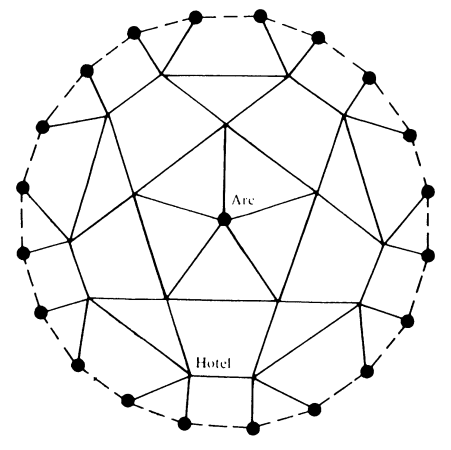
\includegraphics[height = 6cm]{paris.png}
%     \end{center}
%     Find the probability that she reaches the Arc de Triomphe before she reaches the outskirts of town
% \end{problem}
% \end{document}


%----------------------------------------------------------------------------------------
%	BIBLIOGRAPHY
%----------------------------------------------------------------------------------------

%\chapter*{Bibliography}
%\addcontentsline{toc}{chapter}{\textcolor{ocre}{Bibliography}} % Add a Bibliography heading to the table of contents

%------------------------------------------------

%\section*{Articles}
%\addcontentsline{toc}{section}{Articles}
%\printbibliography[heading=bibempty,type=article]

%------------------------------------------------

%\section*{Books}
%\addcontentsline{toc}{section}{Books}
%\printbibliography[heading=bibempty,type=book]

%----------------------------------------------------------------------------------------
%	INDEX
%----------------------------------------------------------------------------------------

\cleardoublepage % Make sure the index starts on an odd (right side) page
\phantomsection
\setlength{\columnsep}{0.75cm} % Space between the 2 columns of the index
\addcontentsline{toc}{chapter}{\textcolor{ocre}{Index}} % Add an Index heading to the table of contents
\printindex % Output the index

%----------------------------------------------------------------------------------------

